%%%%%%%%%%%%%%%%%%%%%%%%%%%%%%%%%%%%%%%%%
% Beamer Presentation
% LaTeX Template
% Version 1.0 (10/11/12)
%
% This template has been downloaded from:
% http://www.LaTeXTemplates.com
%
% License:
% CC BY-NC-SA 3.0 (http://creativecommons.org/licenses/by-nc-sa/3.0/)
%
%%%%%%%%%%%%%%%%%%%%%%%%%%%%%%%%%%%%%%%%%

%----------------------------------------------------------------------------------------
%	PACKAGES AND THEMES
%----------------------------------------------------------------------------------------

\documentclass{beamer}

\mode<presentation> {

% The Beamer class comes with a number of default slide themes
% which change the colors and layouts of slides. Below this is a list
% of all the themes, uncomment each in turn to see what they look like.

\usetheme{default}
%\usetheme{AnnArbor}
%\usetheme{Antibes}
%\usetheme{Bergen}
%\usetheme{Berkeley}
%\usetheme{Berlin}
%\usetheme{Boadilla}
%\usetheme{CambridgeUS}
%\usetheme{Copenhagen}
%\usetheme{Darmstadt}
%\usetheme{Dresden}
%\usetheme{Frankfurt}
%\usetheme{Goettingen}
%\usetheme{Hannover}
%\usetheme{Ilmenau}
%\usetheme{JuanLesPins}
%\usetheme{Luebeck}
%\usetheme{Madrid}
%\usetheme{Malmoe}
%\usetheme{Marburg}
%\usetheme{Montpellier}
%\usetheme{PaloAlto}
%\usetheme{Pittsburgh}
%\usetheme{Rochester}
%\usetheme{Singapore}
%\usetheme{Szeged}
%\usetheme{Warsaw}

% As well as themes, the Beamer class has a number of color themes
% for any slide theme. Uncomment each of these in turn to see how it
% changes the colors of your current slide theme.

%\usecolortheme{albatross}
%\usecolortheme{beaver}
%\usecolortheme{beetle}
%\usecolortheme{crane}
%\usecolortheme{dolphin}
%\usecolortheme{dove}
%\usecolortheme{fly}
%\usecolortheme{lily}
%\usecolortheme{orchid}
%\usecolortheme{rose}
%\usecolortheme{seagull}
%\usecolortheme{seahorse}
%\usecolortheme{whale}
%\usecolortheme{wolverine}

%\setbeamertemplate{footline} % To remove the footer line in all slides uncomment this line
%\setbeamertemplate{footline}[page number] % To replace the footer line in all slides with a simple slide count uncomment this line

%\setbeamertemplate{navigation symbols}{} % To remove the navigation symbols from the bottom of all slides uncomment this line
}

\usepackage{graphicx} % Allows including images
\usepackage{booktabs} % Allows the use of \toprule, \midrule and \bottomrule in tables
\usepackage{tikz}

%----------------------------------------------------------------------------------------
%	TITLE PAGE
%----------------------------------------------------------------------------------------

\title[Short title]{Spectral Image Analysis for \\Medical Imaging} % The short title appears at the bottom of every slide, the full title is only on the title page

\author{Michael Painter} % Your name
\institute[UoC] % Your institution as it will appear on the bottom of every slide, may be shorthand to save space
{
University of Cambridge \\ % Your institution for the title page
\medskip
\textit{mp703@cam.ac.uk} % Your email address
}
\date{4th February 2016} % Date, can be changed to a custom date

\begin{document}

\begin{frame}
\titlepage % Print the title page as the first slide
\end{frame}

%----------------------------------------------------------------------------------------
%	PRESENTATION SLIDES
%----------------------------------------------------------------------------------------

\begin{frame}
    \frametitle{Overview of Proejct - What am I doing?}

    \begin{itemize}
        \item Investigating use of \textit{spectral images} for medical imaging. 
        \item An image becomes a \textit{data cube} $I(x,y,\lambda)$. (E.g. $\lambda \in \{R, G, B\}$).
        \item Aim to provide a pixel labelling/image segmentation for medical images using spectral information.
        \item We will use machine learning.
        \item Two approaches: Neural Nets, Random Forests.
    \end{itemize}
\end{frame}

%------------------------------------------------


\begin{frame}
    \frametitle{Random Forests}

    \begin{block}{DecisionForests}
        \begin{itemize}
            \item Forest = set of trees.
            \item Trees `vote' towards a winning class.
        \end{itemize}

        \begin{figure}[H]
            \centering
            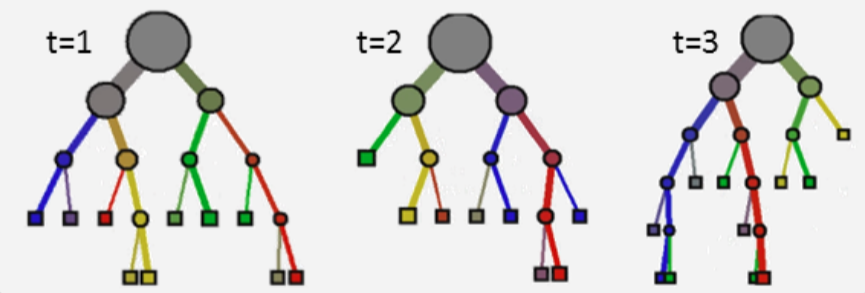
\includegraphics[scale=0.25]{Forests.png}
            \caption{}
        \end{figure}
    \end{block}
\end{frame}

\begin{frame}
    \frametitle{Random Forests}

    \begin{block}{The random bit}
        \begin{itemize}
            \item Use \textit{weak learners} to split the training sequence up.
            \item Want the split that leads to the optimal \textit{information gain}.
            \item Can't possibly try every way of splitting.
        \end{itemize}

        \begin{figure}[H]
            \centering
            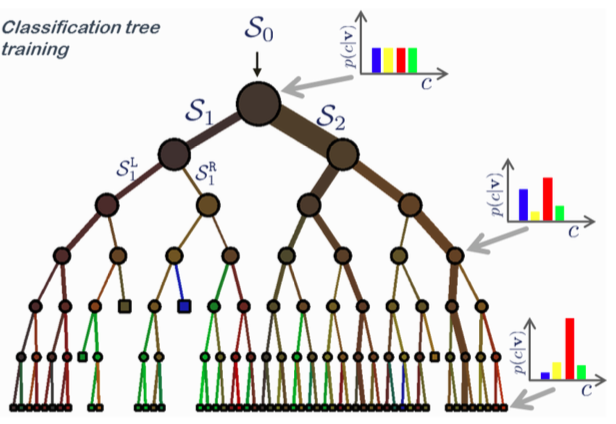
\includegraphics[scale=0.3]{ProbabilityTree.png}
            \caption{}
        \end{figure}
    \end{block}
\end{frame}

\begin{frame}
    \frametitle{Progress}

    \begin{block}{Completed}
        \begin{itemize}
            \item Random forests library.
            \item `DataCube' interface.
            \item Pixel labelling using random forests,
            \item and using Encog. (A machine learning library in Java with Neural Nets).
        \end{itemize}
    \end{block}
\end{frame}

\begin{frame}
    \frametitle{Progress}

    \begin{figure}[H]
        \centering
        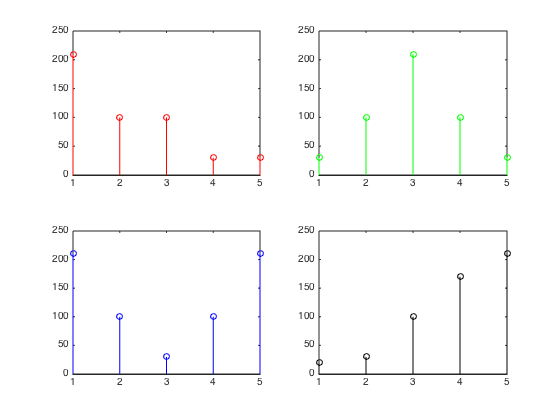
\includegraphics[scale=0.3]{toyImageProfiles.png}
    \end{figure}

    \begin{columns}[c]
        \column{.47\textwidth} % Left column and width
        
\includegraphics[scale=0.15]{Interpolated5DimImage1.png} \hspace{0.3pt}
        
\includegraphics[scale=0.15]{Interpolated5DimImage2.png} \hspace{0.3pt}
        
\includegraphics[scale=0.15]{Interpolated5DimImage3.png}\\ \hspace{17pt}
        
\includegraphics[scale=0.15]{Interpolated5DimImage4.png} \hspace{0.3pt}
        
\includegraphics[scale=0.15]{Interpolated5DimImage5.png}

        \column{.08\textwidth}
        $\rightarrow$

        \column{.45\textwidth}
        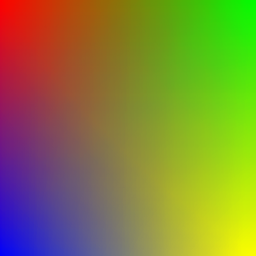
\includegraphics[scale=0.2]{rf.png} \hspace{0.3pt}
        
\includegraphics[scale=0.2]{rf256.png} \\
        
\includegraphics[scale=0.2]{rf1000.png} \hspace{0.3pt}
        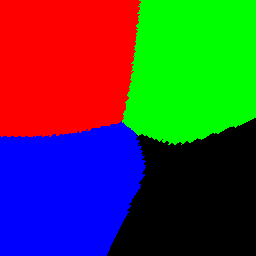
\includegraphics[scale=0.2]{nn.png}
    \end{columns}
\end{frame}

\begin{frame}
    \frametitle{What's next?}

    \begin{itemize}
        \item De noising images with Poisson noise.
        \item Get it working on some real images.
        \item Compare the implementations on how they perform (speed and accuracy).
    \end{itemize}
\end{frame}

\begin{frame}
    \frametitle{What's next?}

        
\includegraphics[height=0.023\textheight]{spatial-denoised/wavelet_den_1.png}
        
\includegraphics[height=0.023\textheight]{spatial-denoised/wavelet_den_2.png}
        
\includegraphics[height=0.023\textheight]{spatial-denoised/wavelet_den_3.png}
        
\includegraphics[height=0.023\textheight]{spatial-denoised/wavelet_den_4.png}
        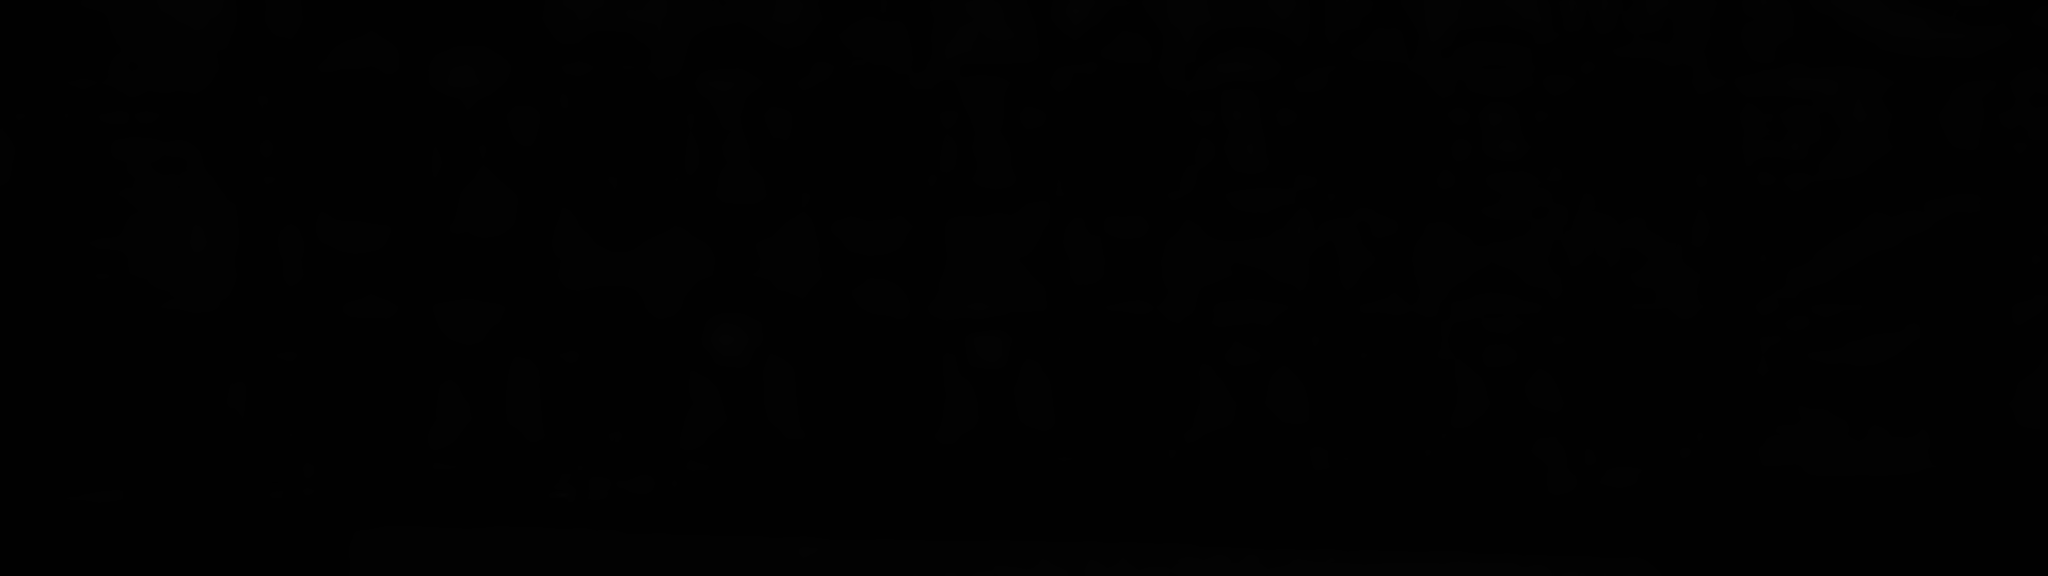
\includegraphics[height=0.023\textheight]{spatial-denoised/wavelet_den_5.png}
        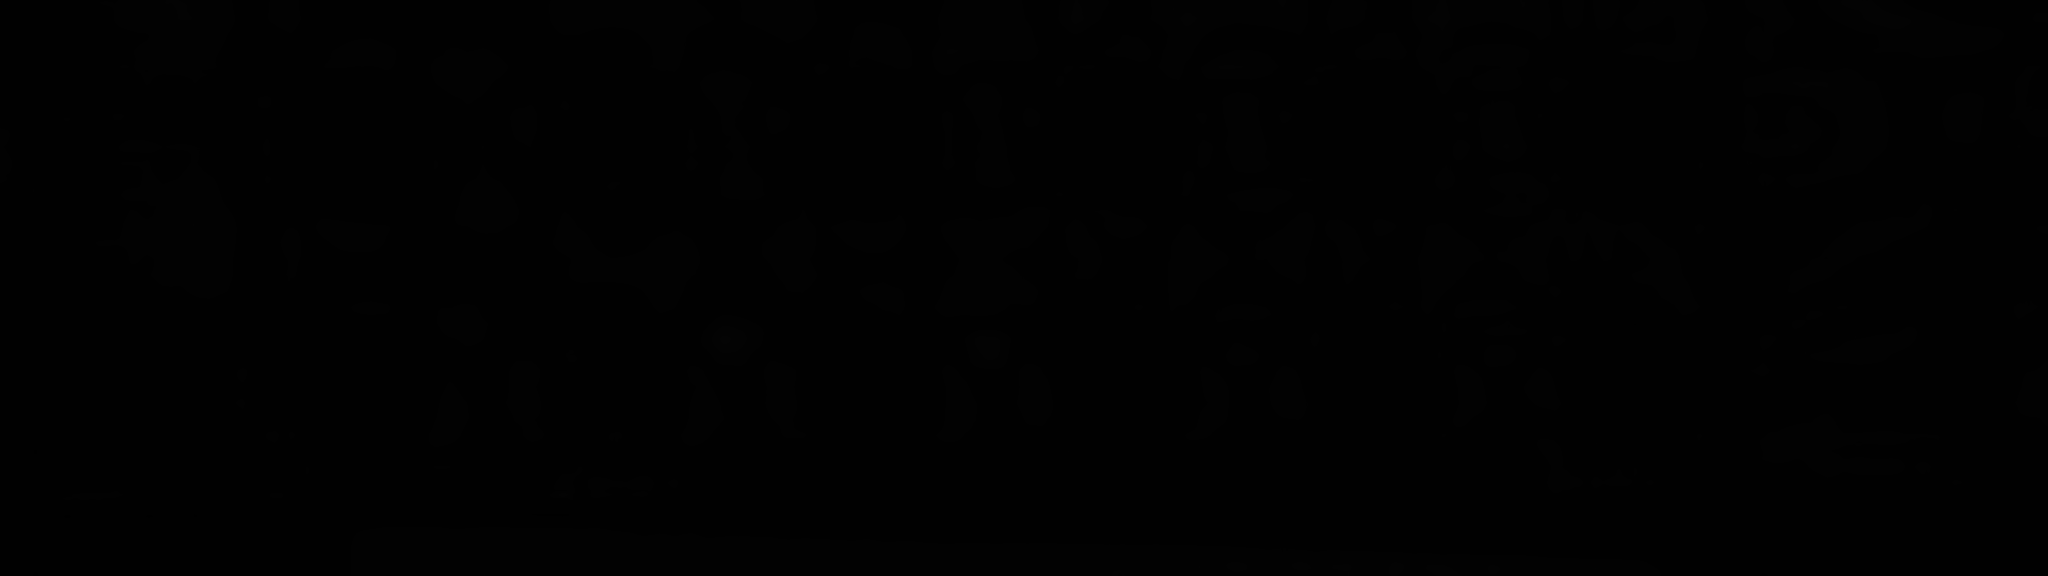
\includegraphics[height=0.023\textheight]{spatial-denoised/wavelet_den_6.png}
        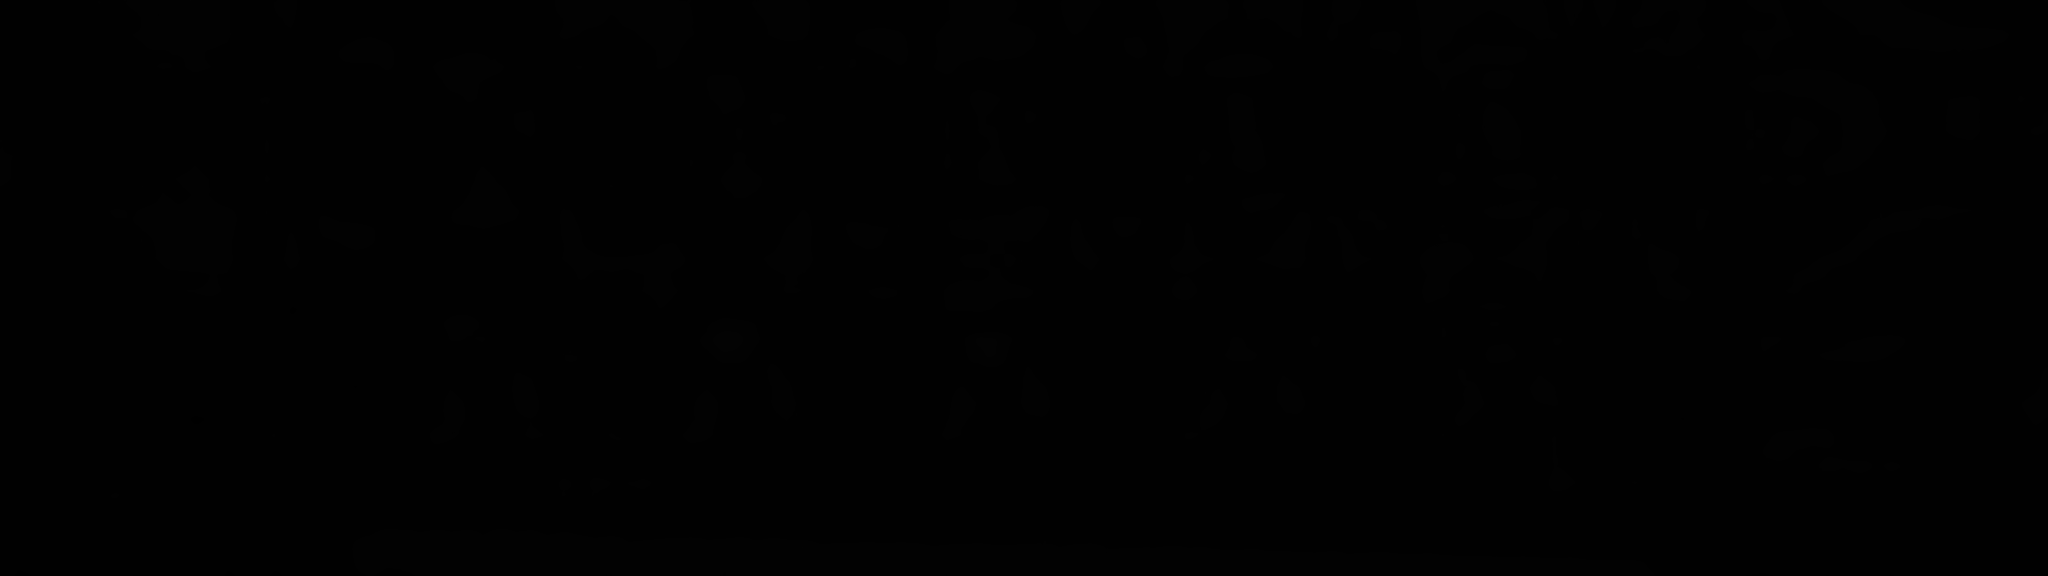
\includegraphics[height=0.023\textheight]{spatial-denoised/wavelet_den_7.png}
        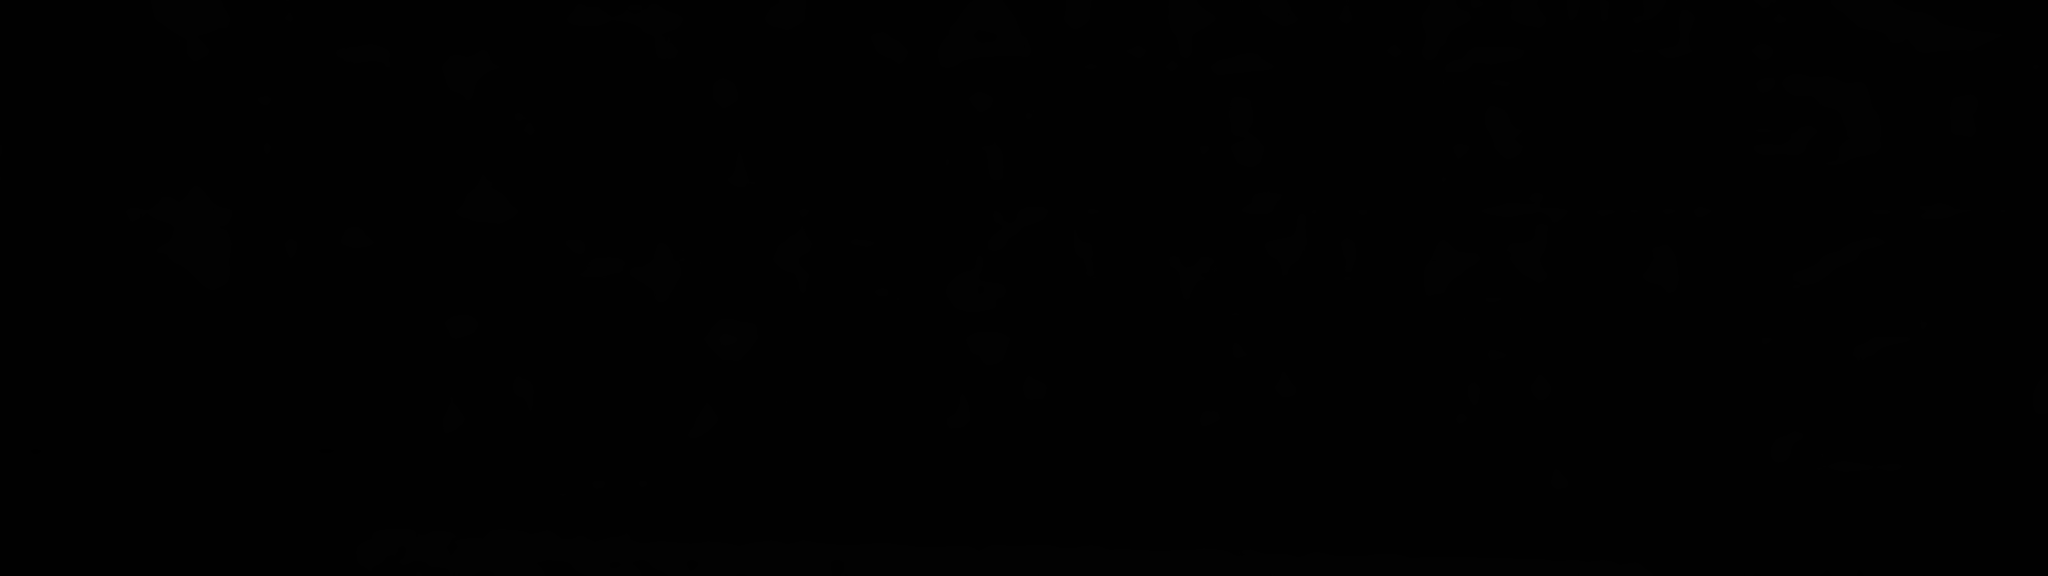
\includegraphics[height=0.023\textheight]{spatial-denoised/wavelet_den_8.png}
        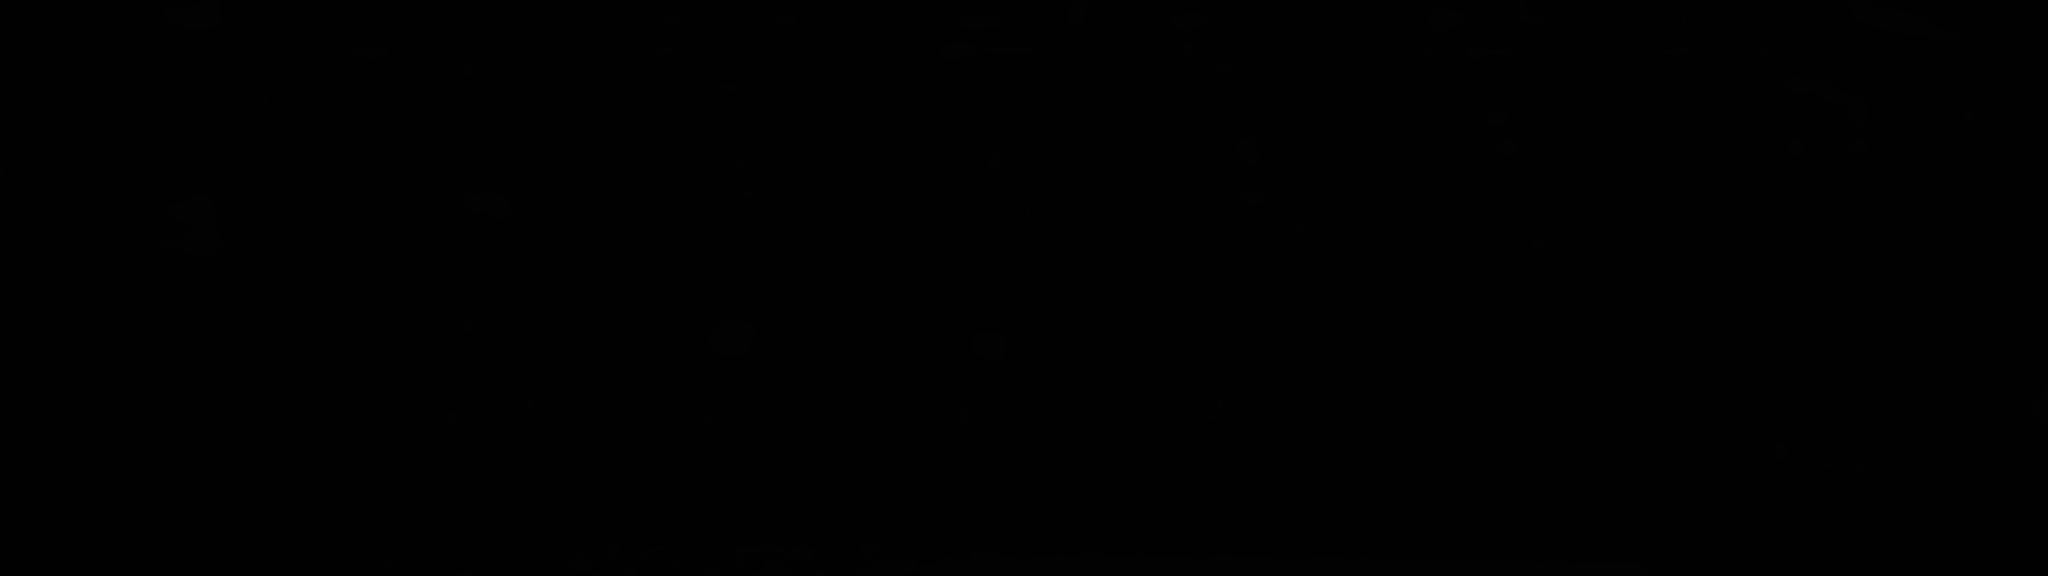
\includegraphics[height=0.023\textheight]{spatial-denoised/wavelet_den_9.png}
        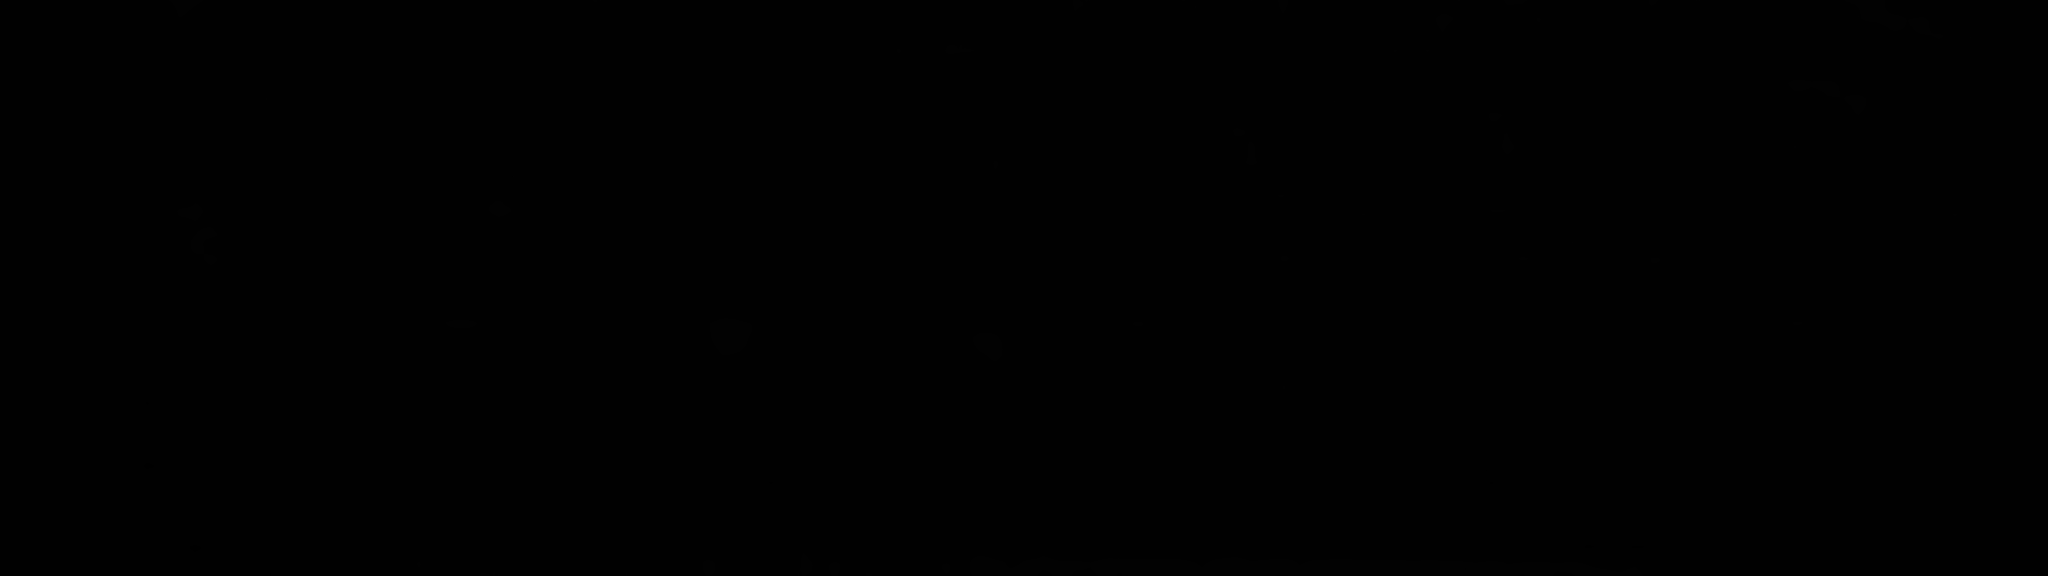
\includegraphics[height=0.023\textheight]{spatial-denoised/wavelet_den_10.png}
        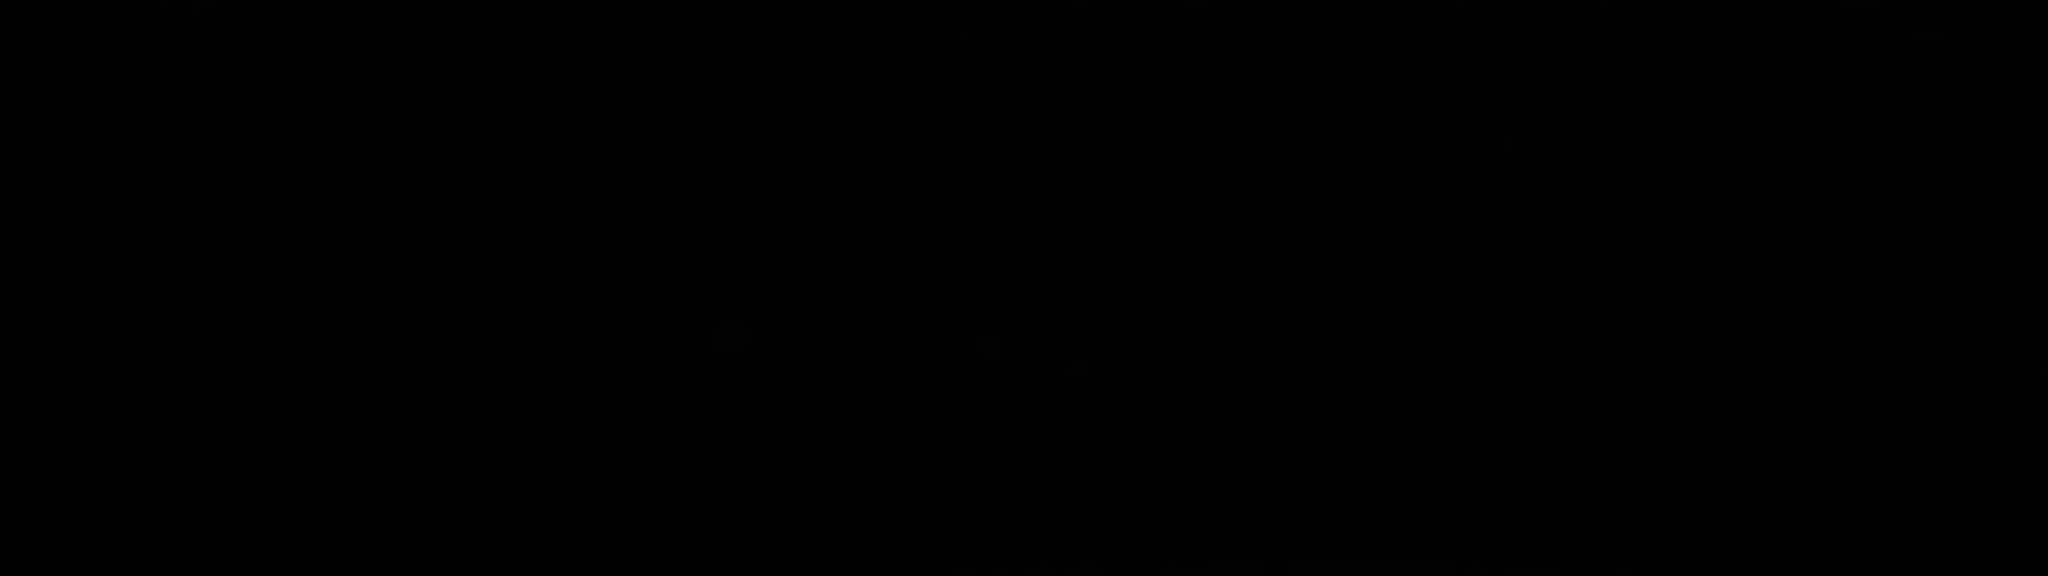
\includegraphics[height=0.023\textheight]{spatial-denoised/wavelet_den_11.png}
        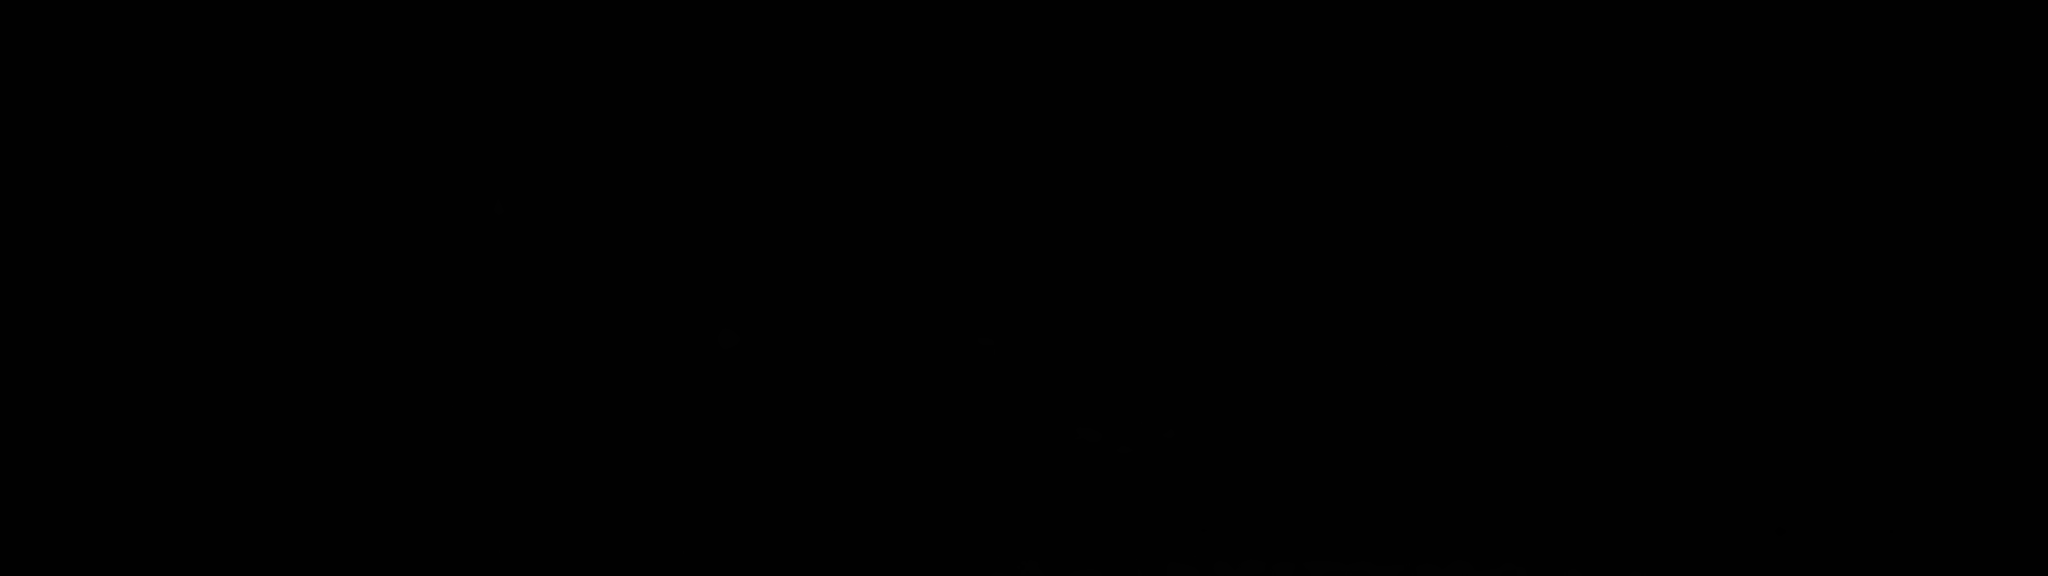
\includegraphics[height=0.023\textheight]{spatial-denoised/wavelet_den_12.png}
        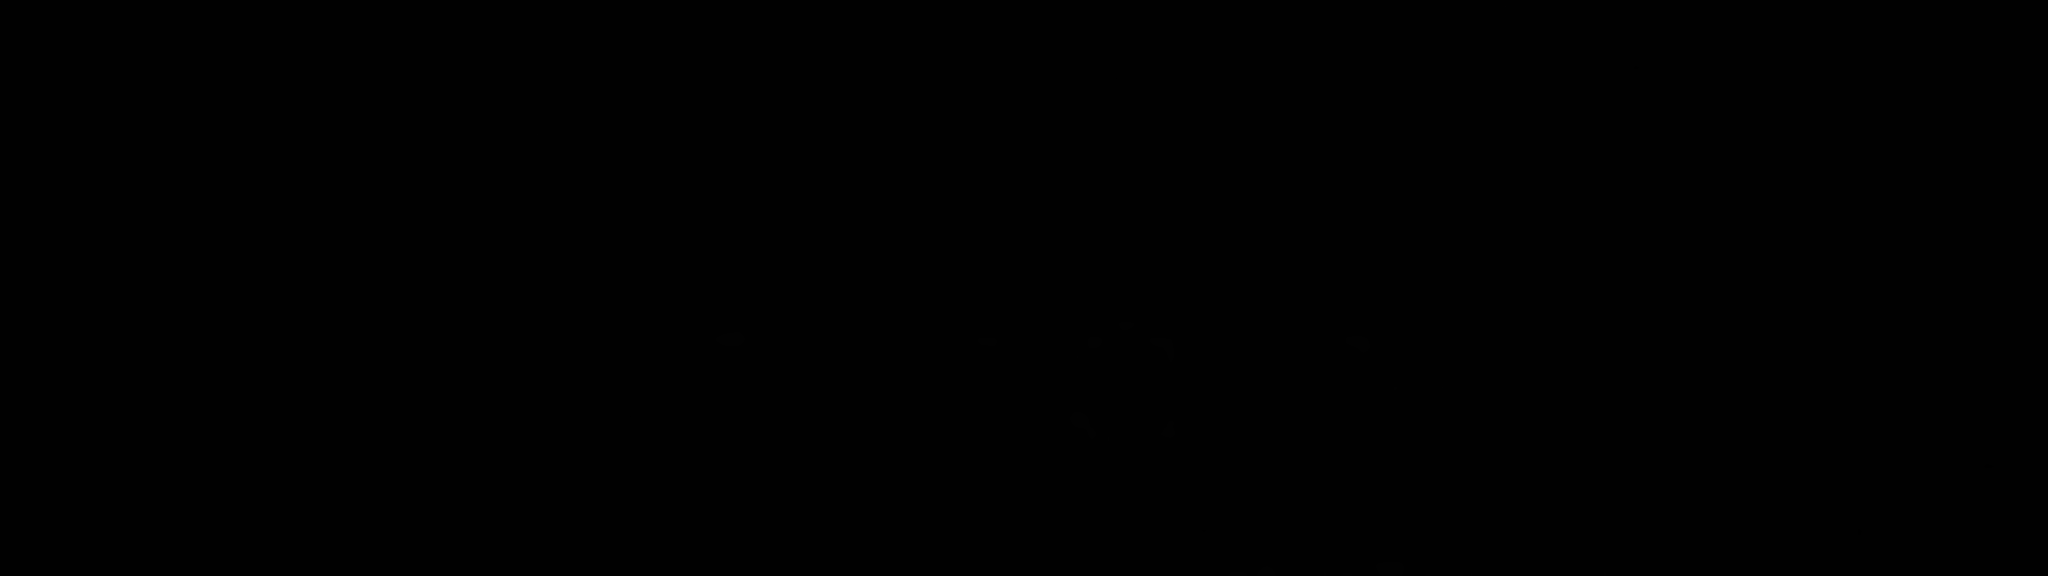
\includegraphics[height=0.023\textheight]{spatial-denoised/wavelet_den_13.png}
        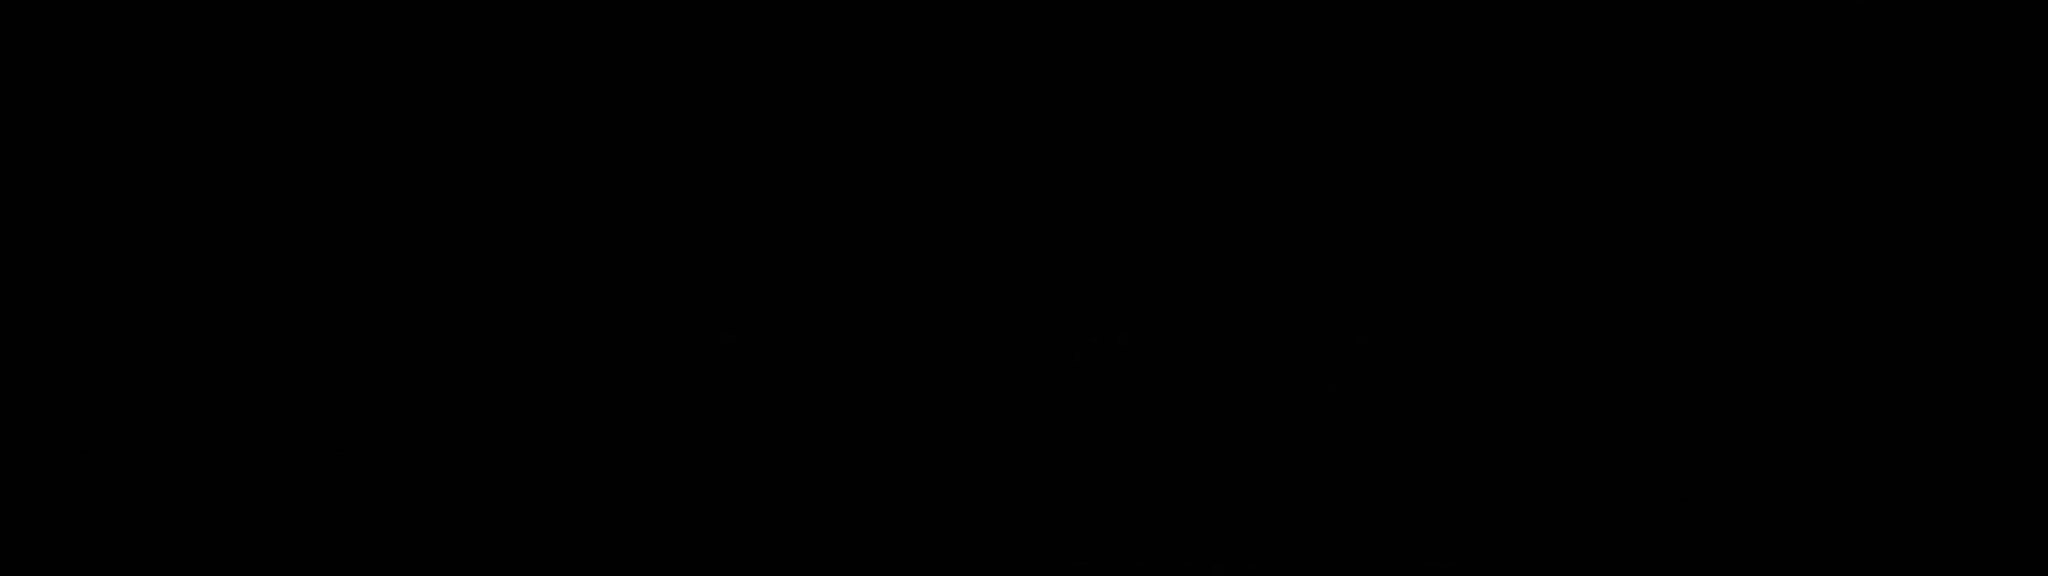
\includegraphics[height=0.023\textheight]{spatial-denoised/wavelet_den_14.png}
        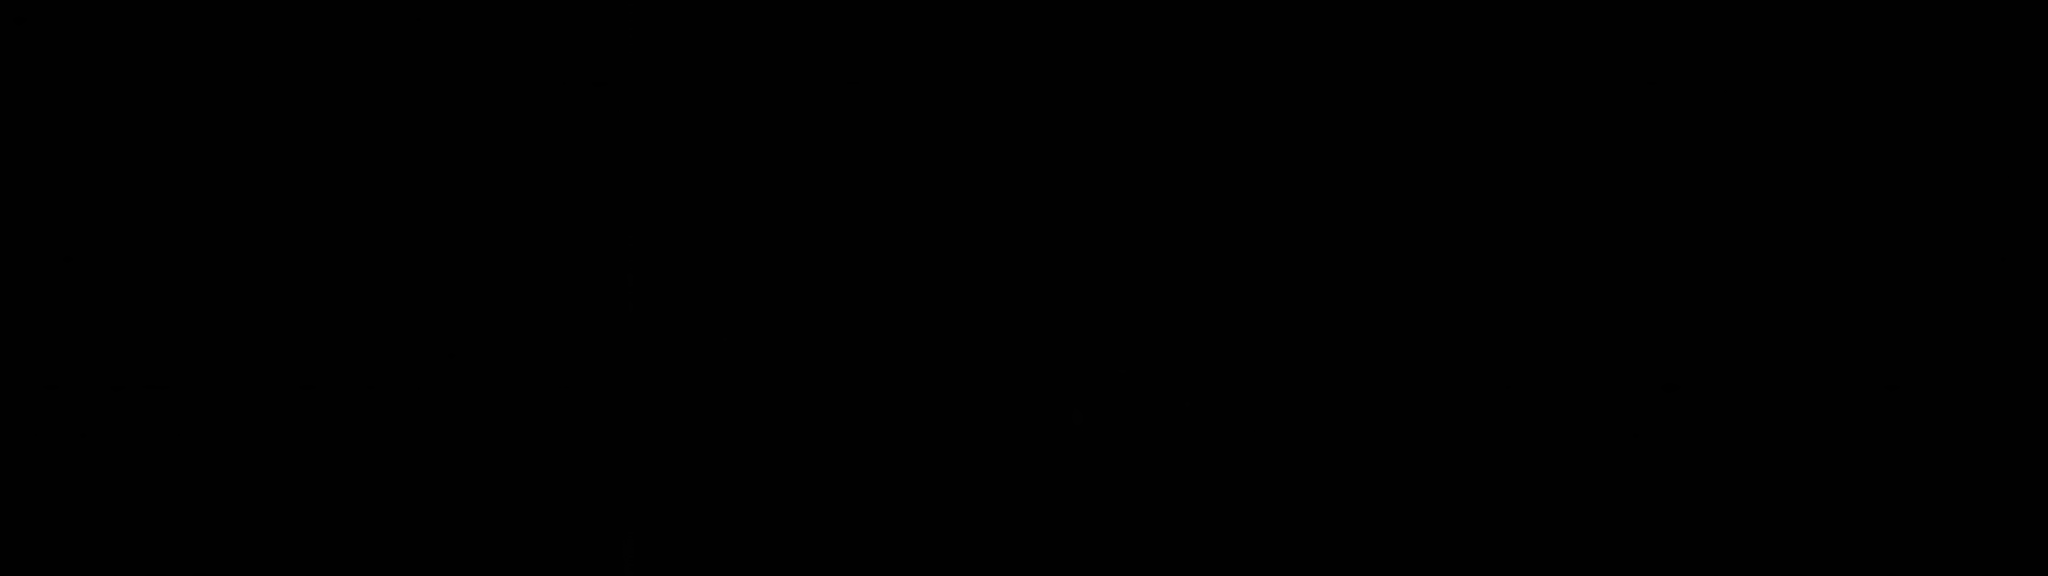
\includegraphics[height=0.023\textheight]{spatial-denoised/wavelet_den_15.png}\\
        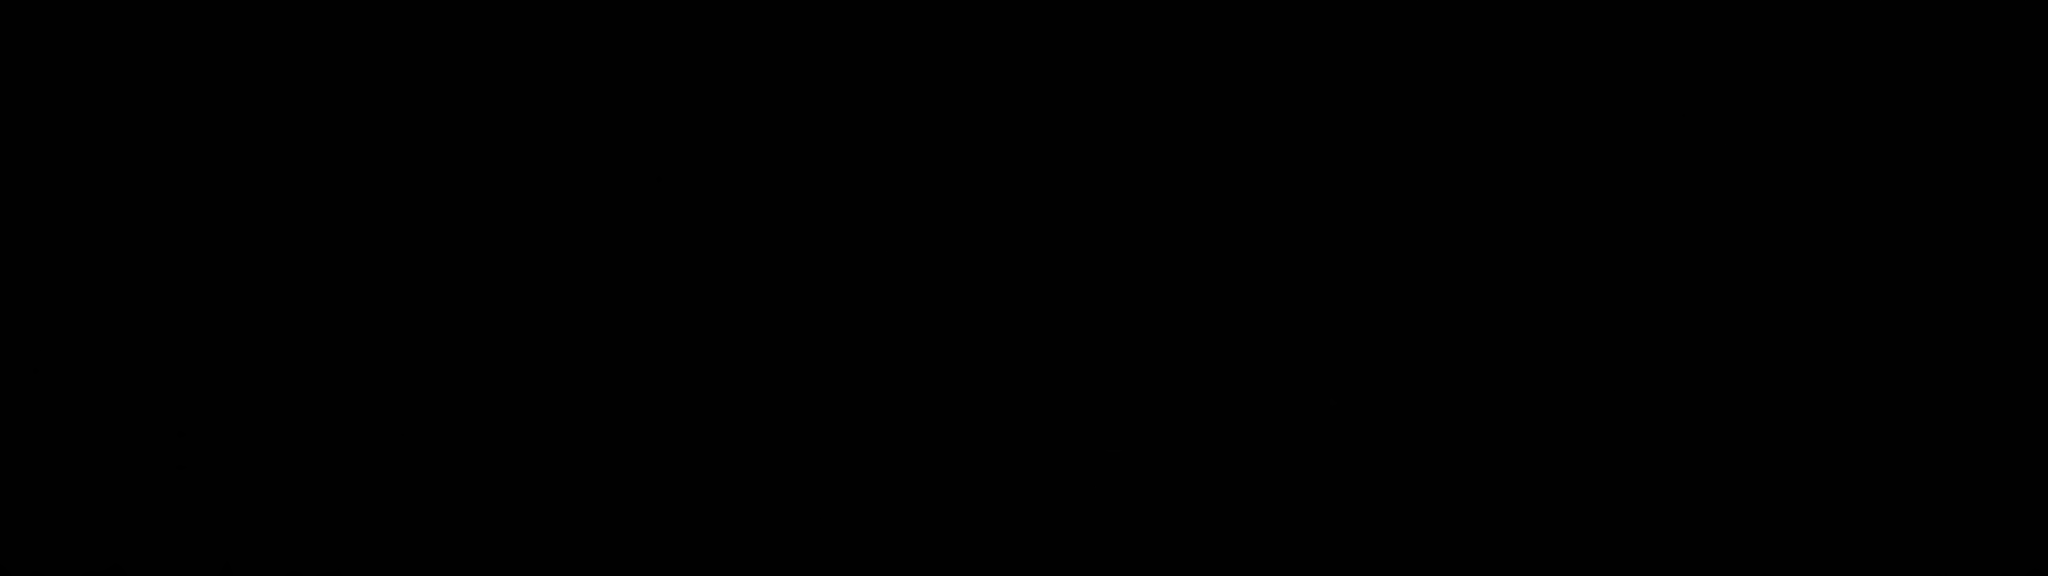
\includegraphics[height=0.023\textheight]{spatial-denoised/wavelet_den_16.png}
        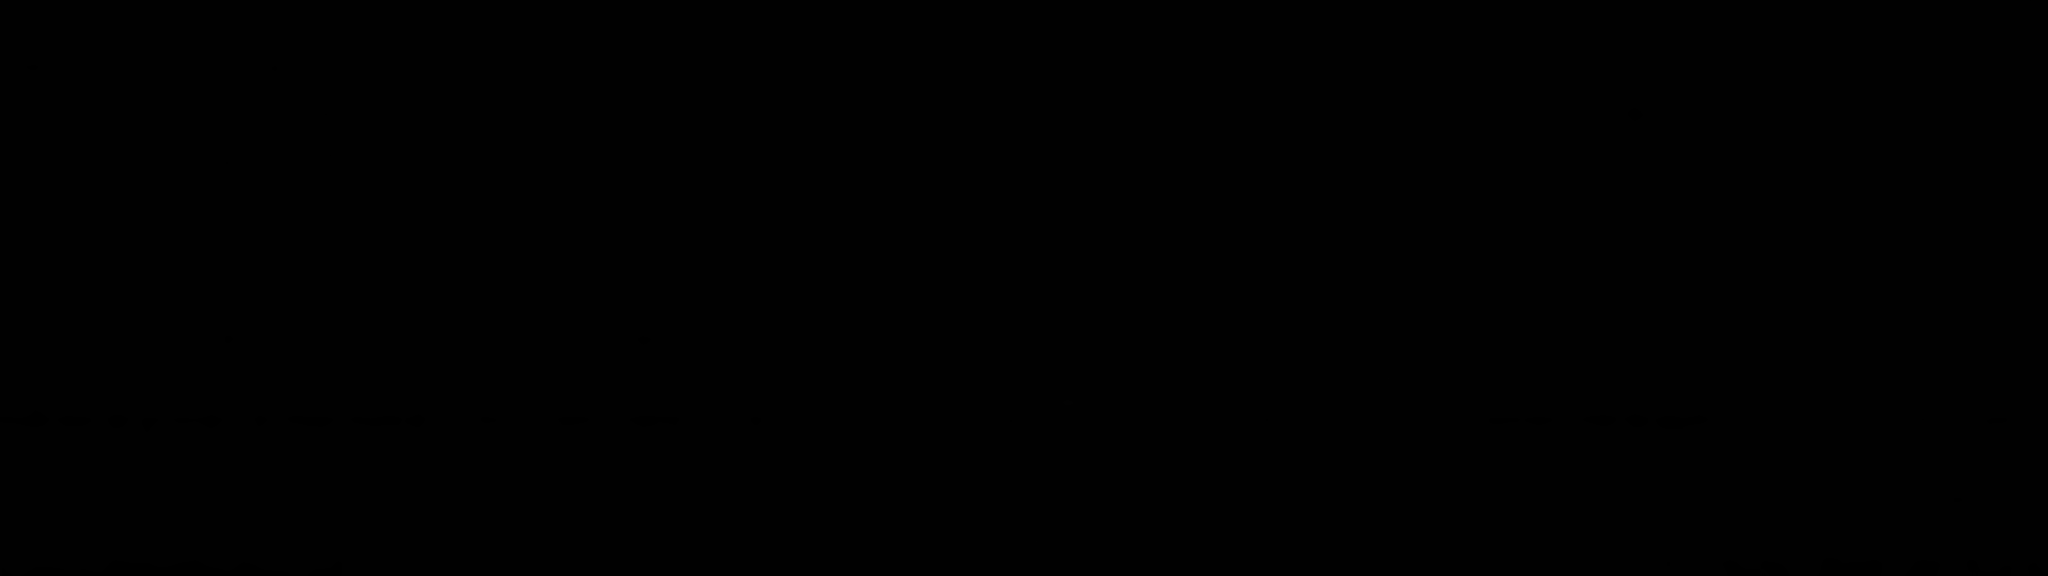
\includegraphics[height=0.023\textheight]{spatial-denoised/wavelet_den_17.png}
        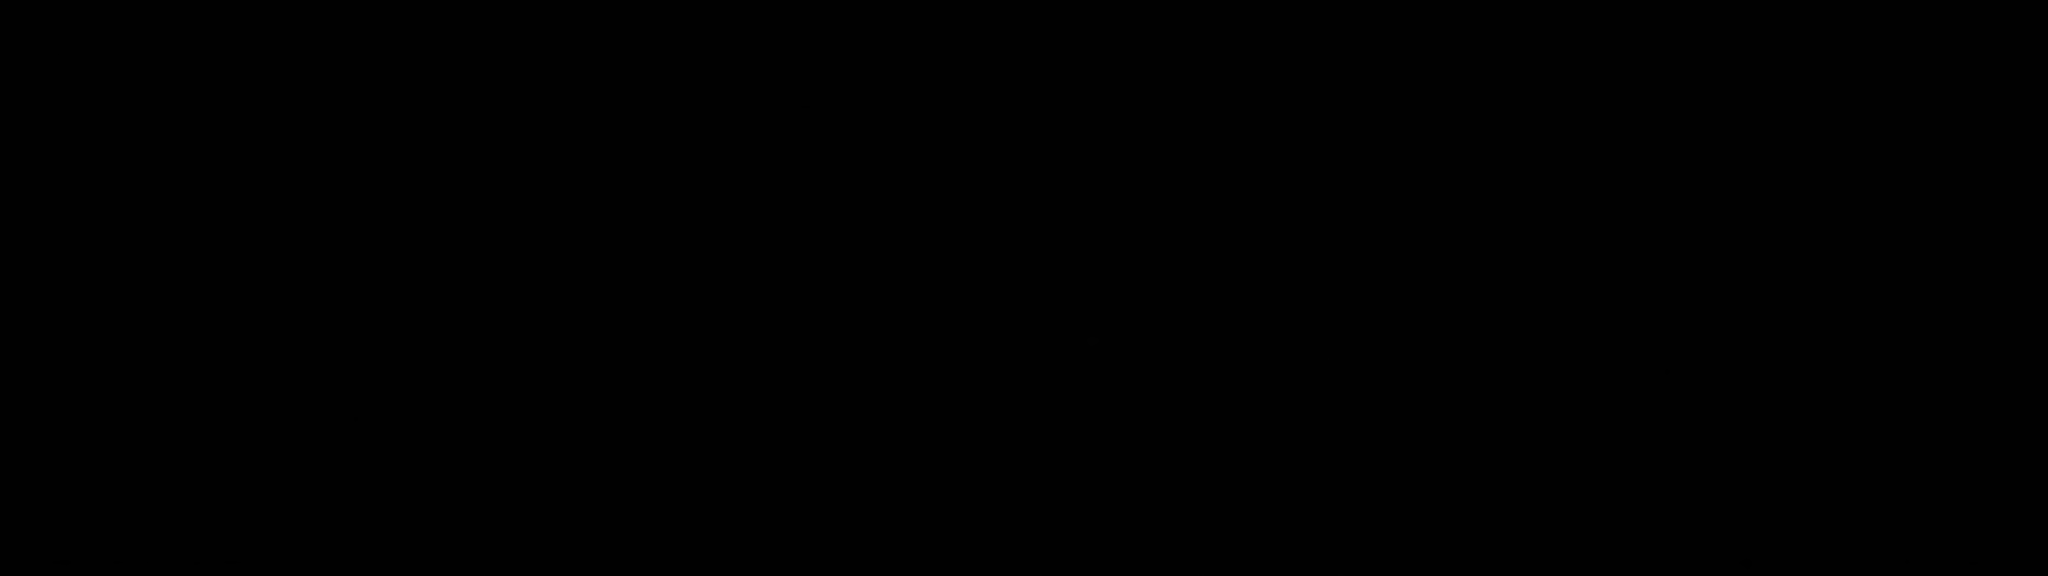
\includegraphics[height=0.023\textheight]{spatial-denoised/wavelet_den_18.png}
        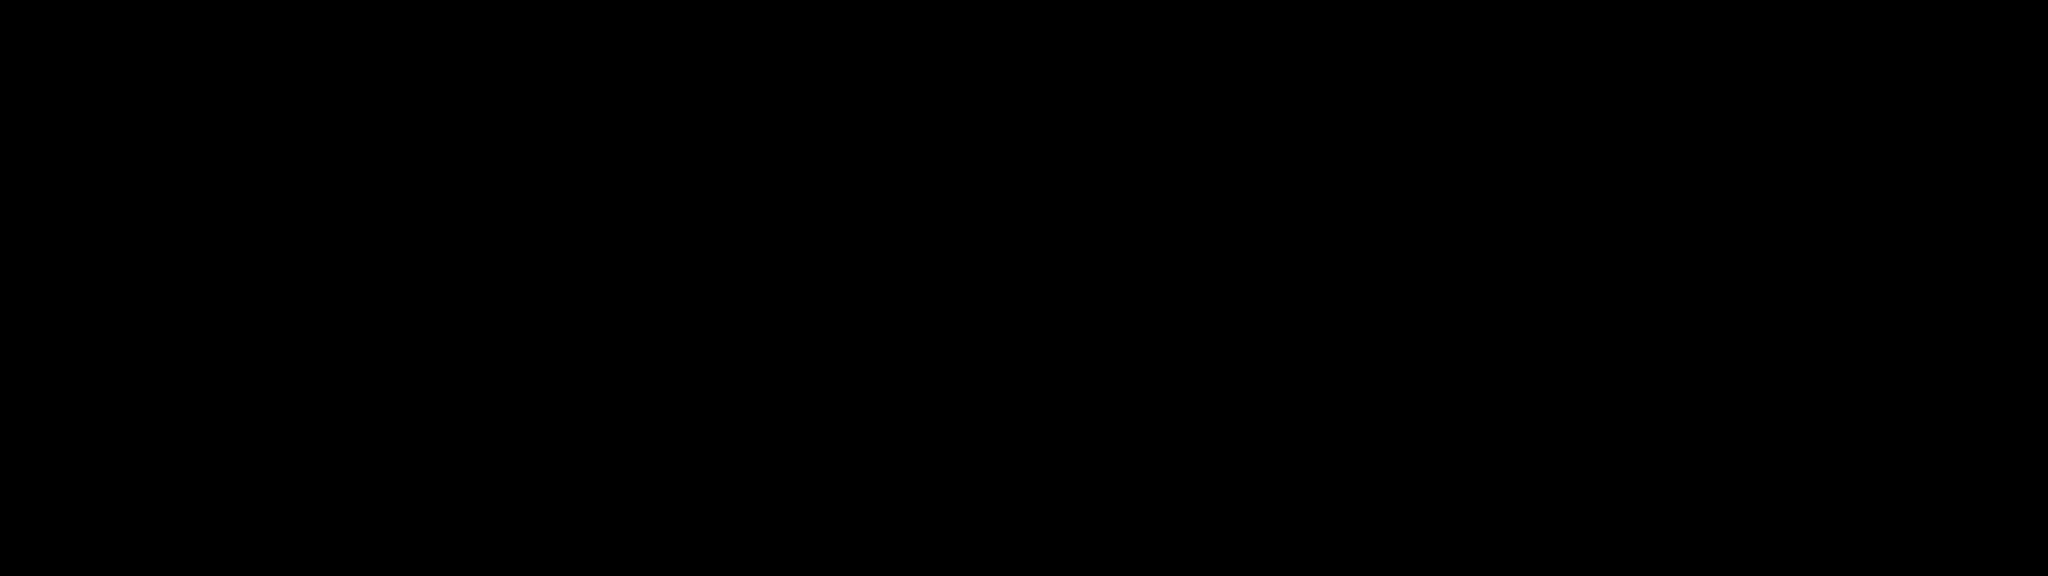
\includegraphics[height=0.023\textheight]{spatial-denoised/wavelet_den_19.png}
        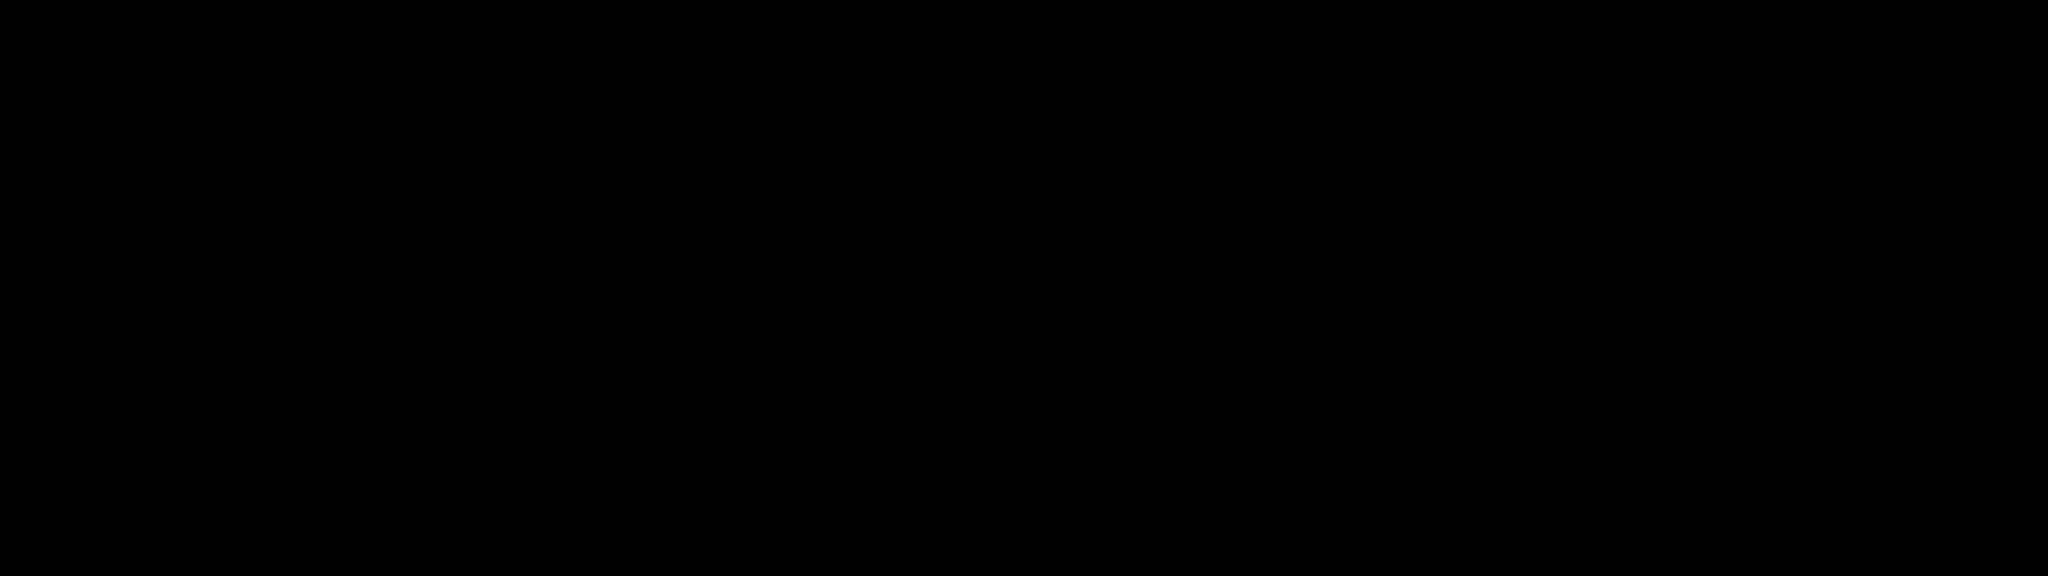
\includegraphics[height=0.023\textheight]{spatial-denoised/wavelet_den_20.png}
        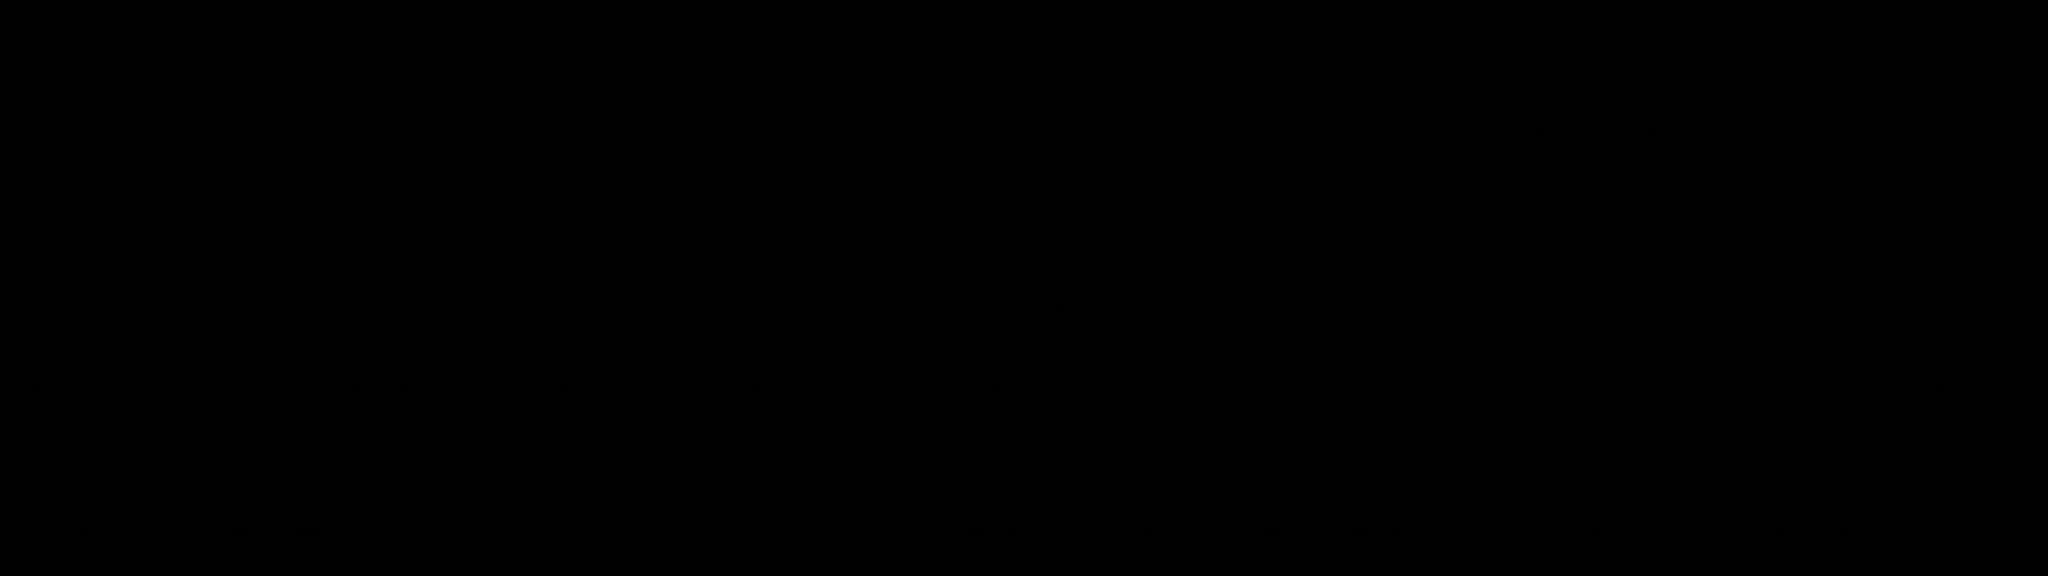
\includegraphics[height=0.023\textheight]{spatial-denoised/wavelet_den_21.png}
        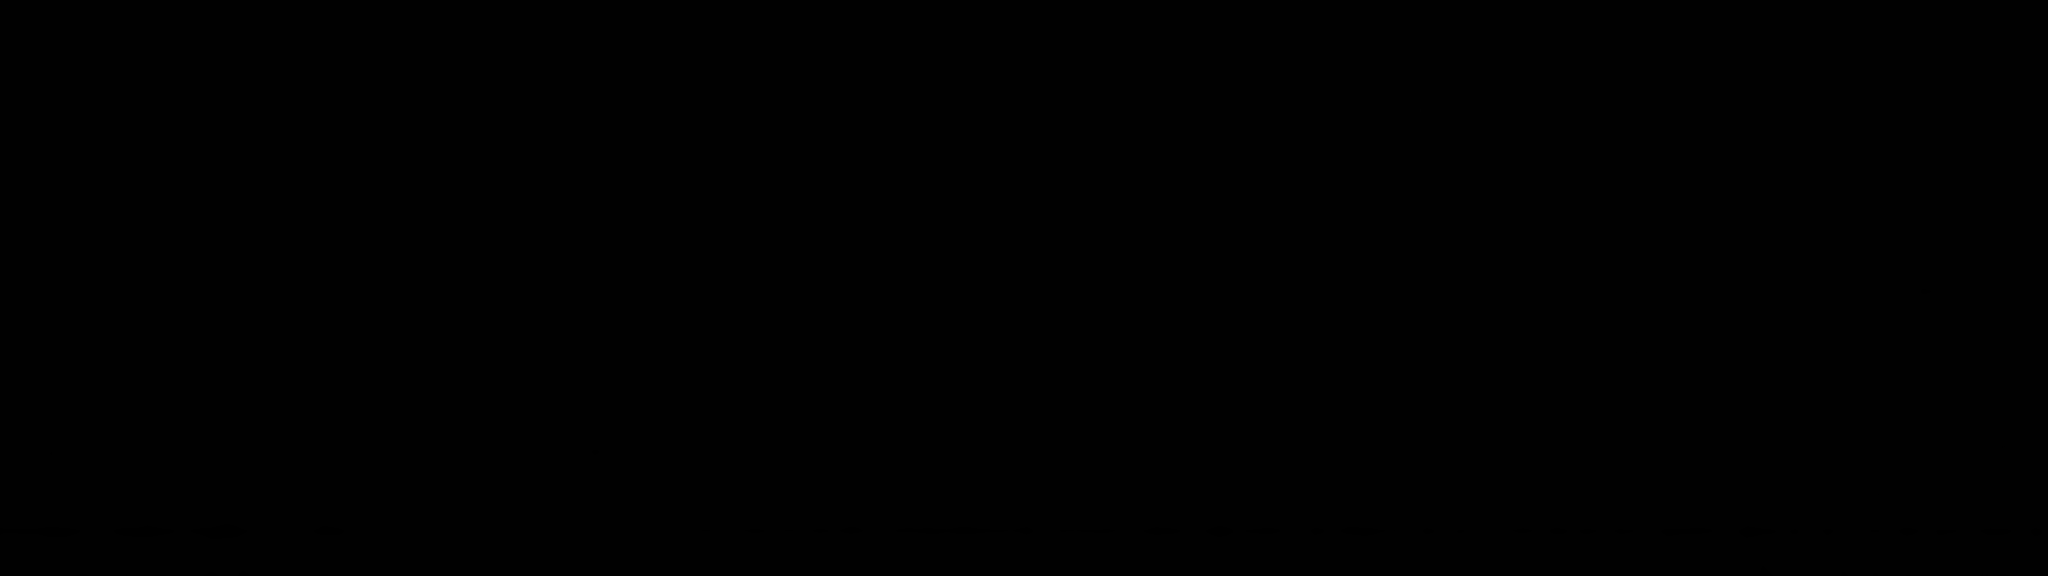
\includegraphics[height=0.023\textheight]{spatial-denoised/wavelet_den_22.png}
        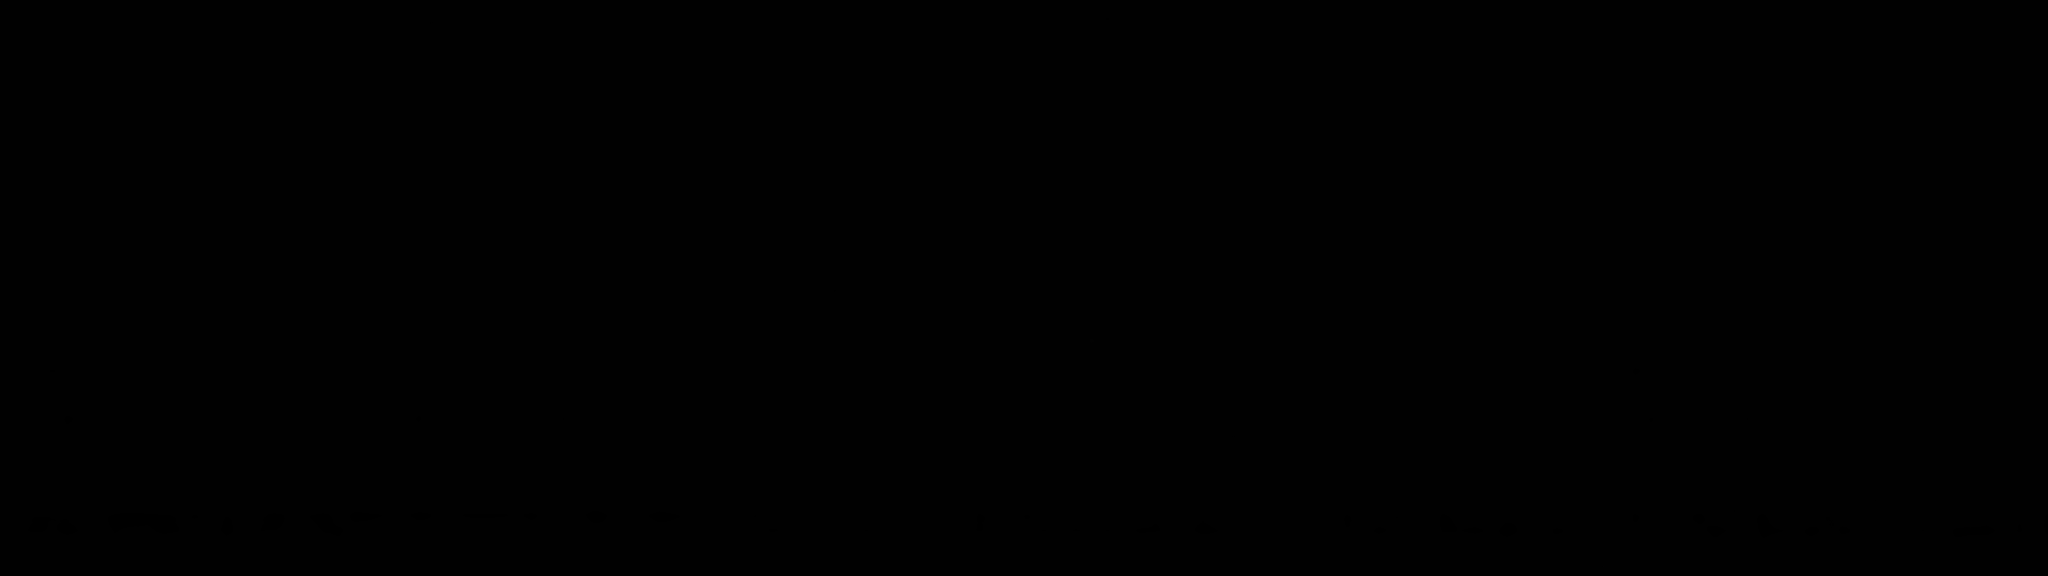
\includegraphics[height=0.023\textheight]{spatial-denoised/wavelet_den_23.png}
        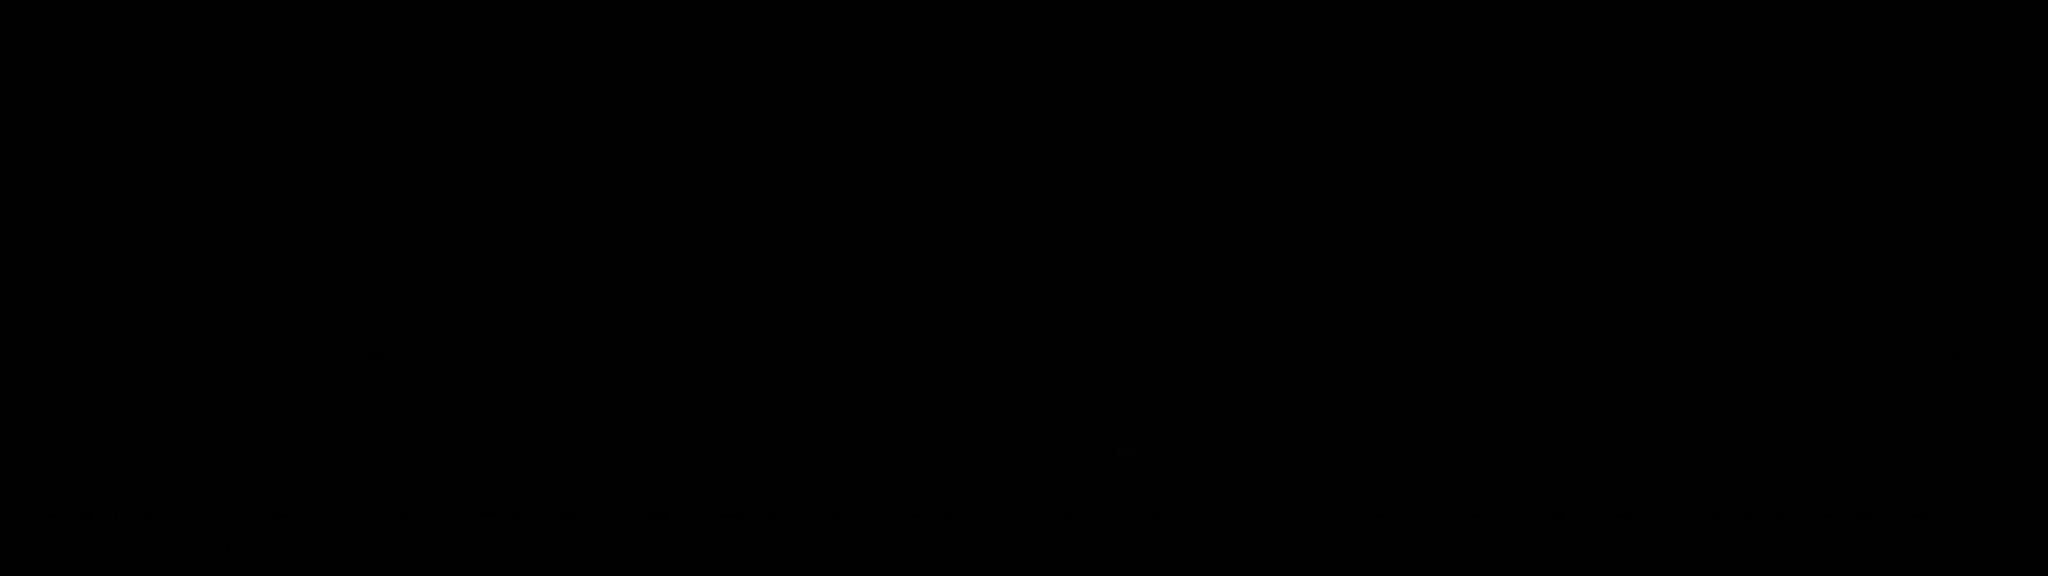
\includegraphics[height=0.023\textheight]{spatial-denoised/wavelet_den_24.png}
        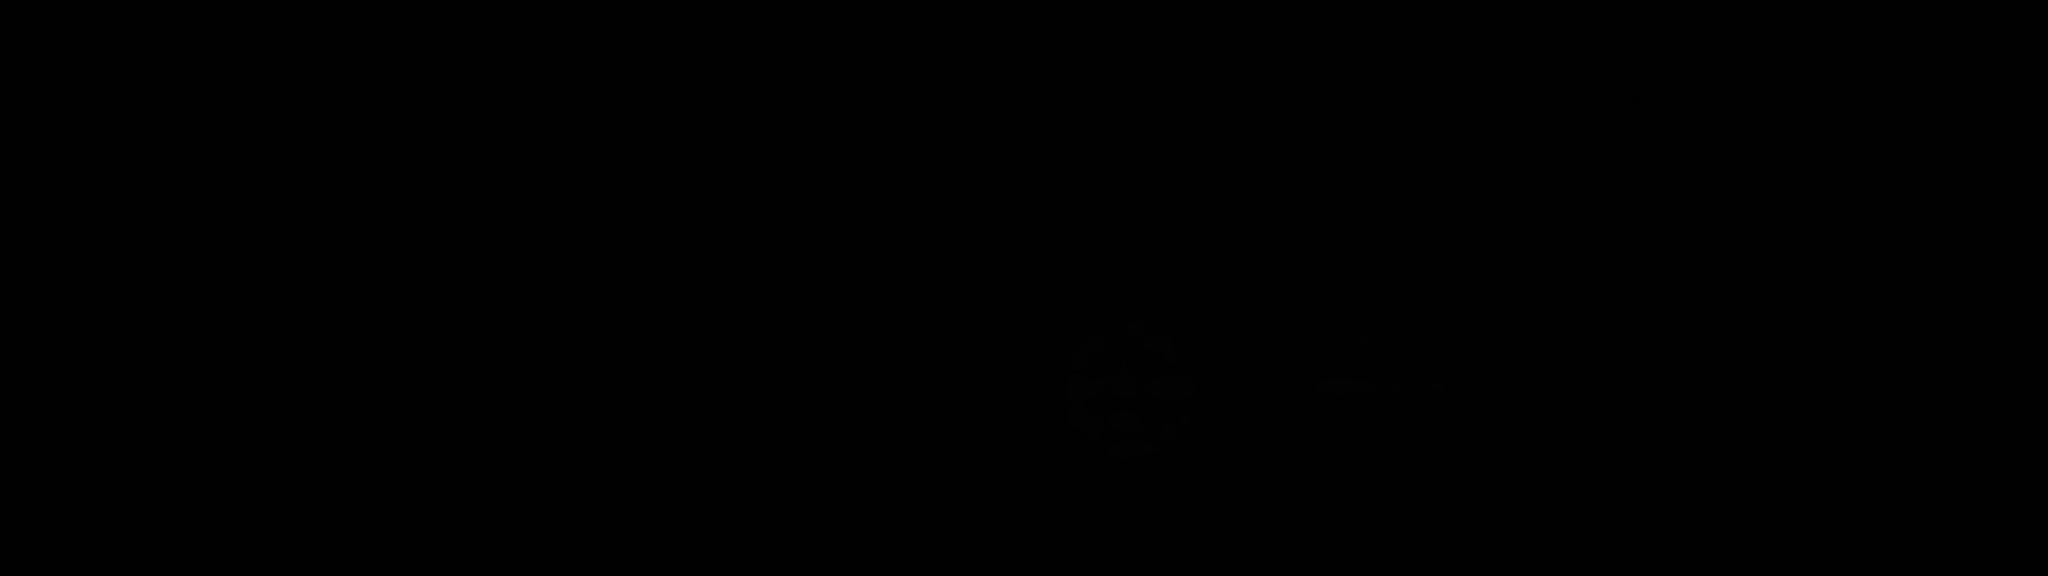
\includegraphics[height=0.023\textheight]{spatial-denoised/wavelet_den_25.png}
        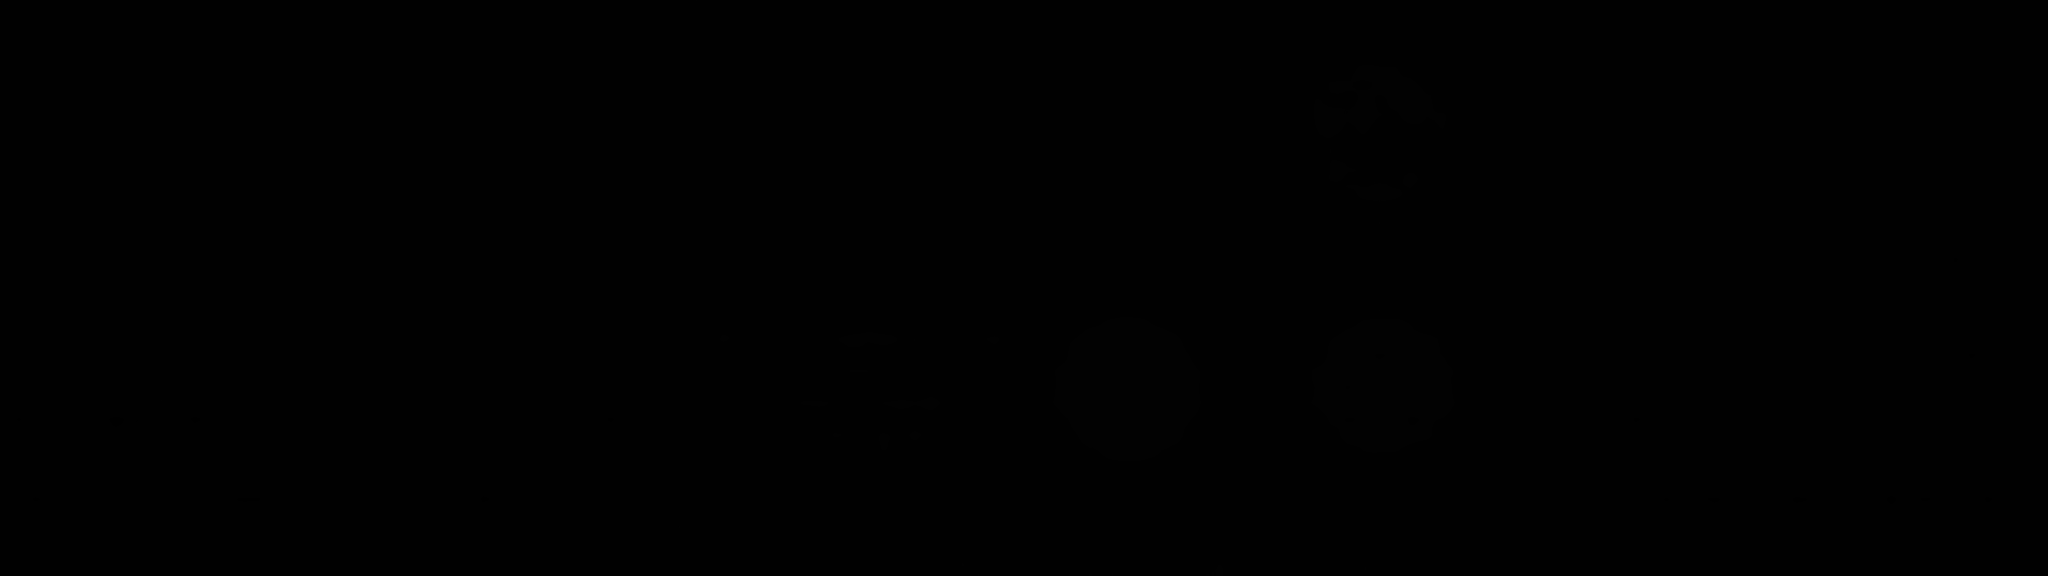
\includegraphics[height=0.023\textheight]{spatial-denoised/wavelet_den_26.png}
        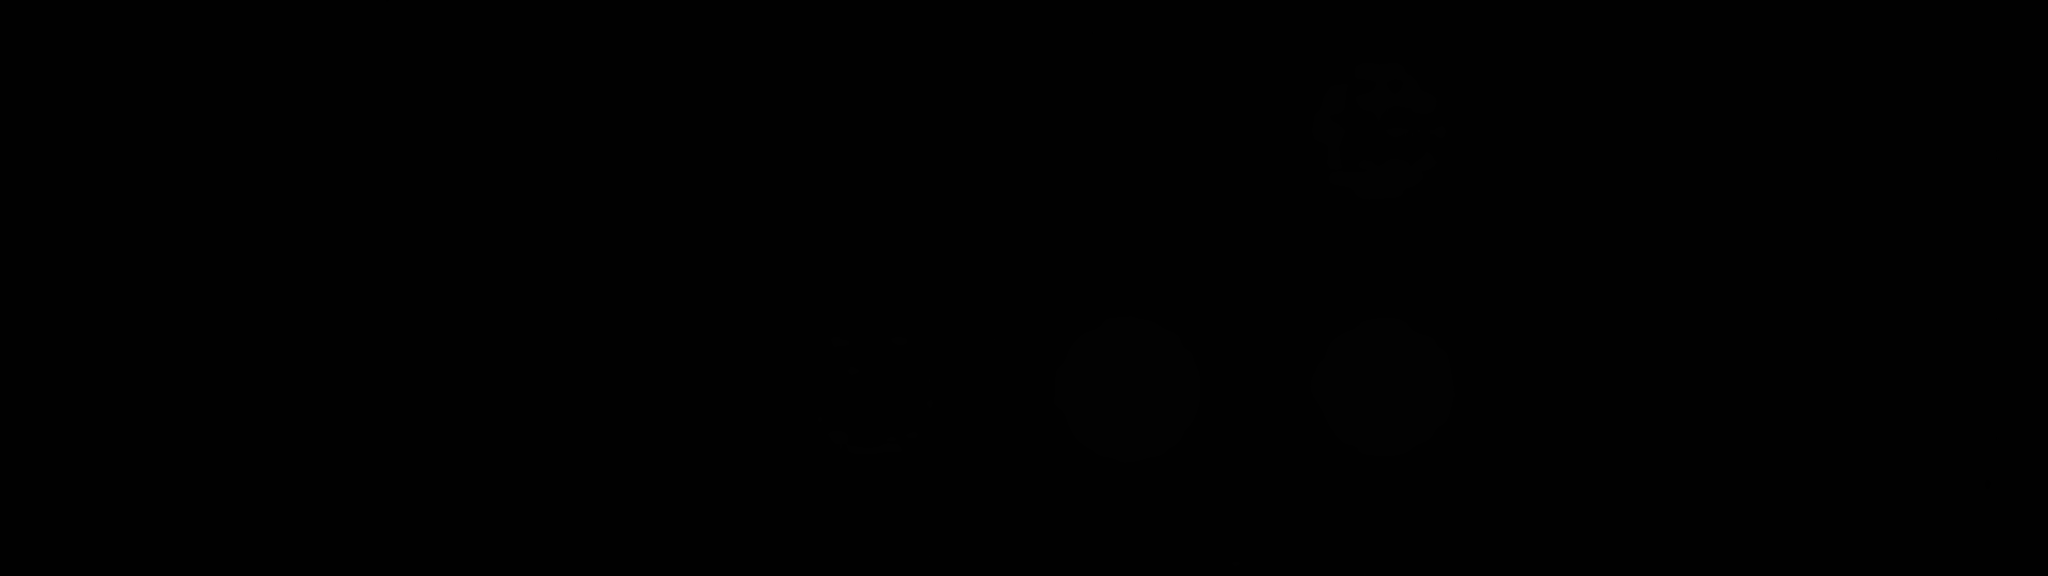
\includegraphics[height=0.023\textheight]{spatial-denoised/wavelet_den_27.png}
        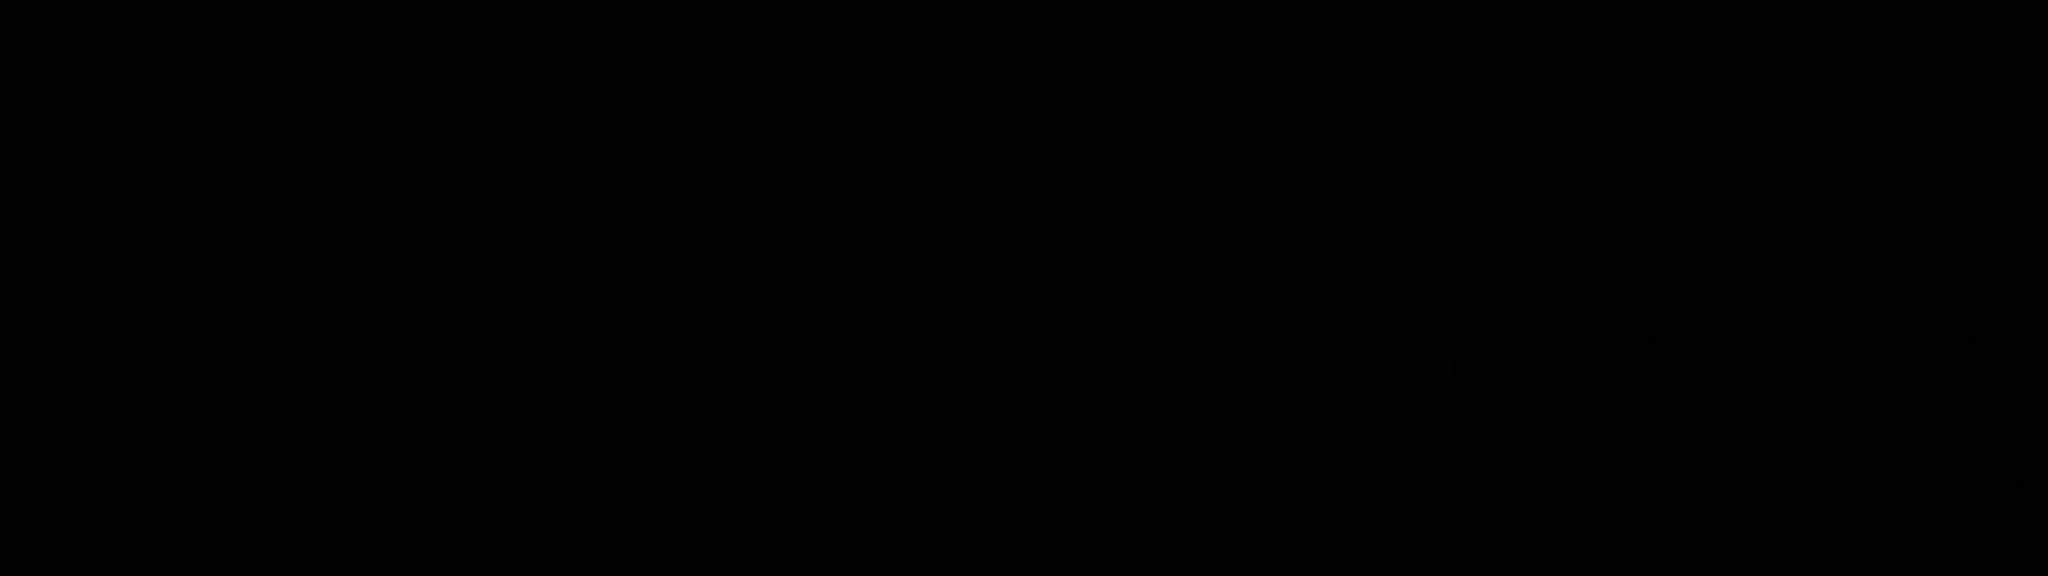
\includegraphics[height=0.023\textheight]{spatial-denoised/wavelet_den_28.png}
        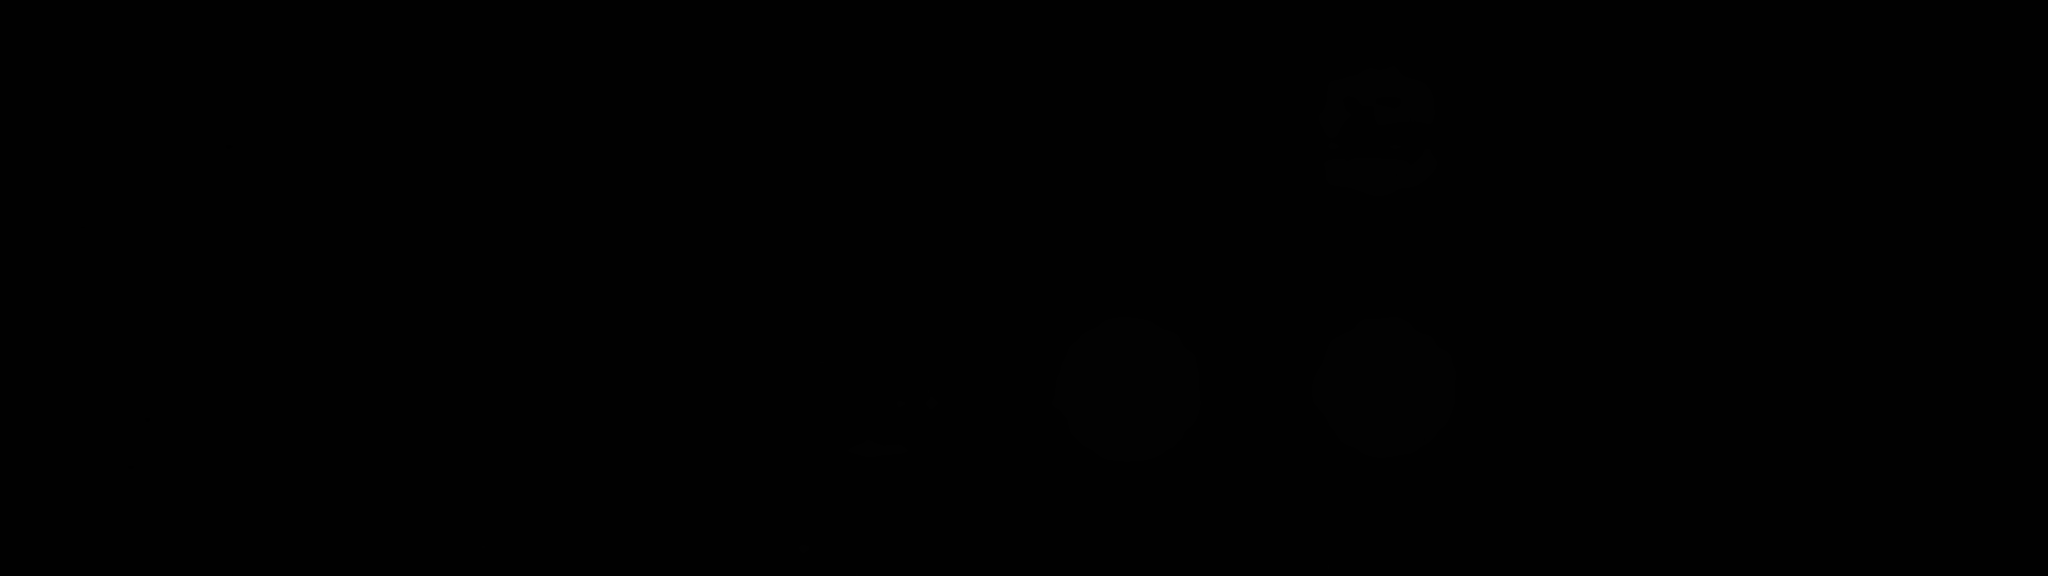
\includegraphics[height=0.023\textheight]{spatial-denoised/wavelet_den_29.png}
        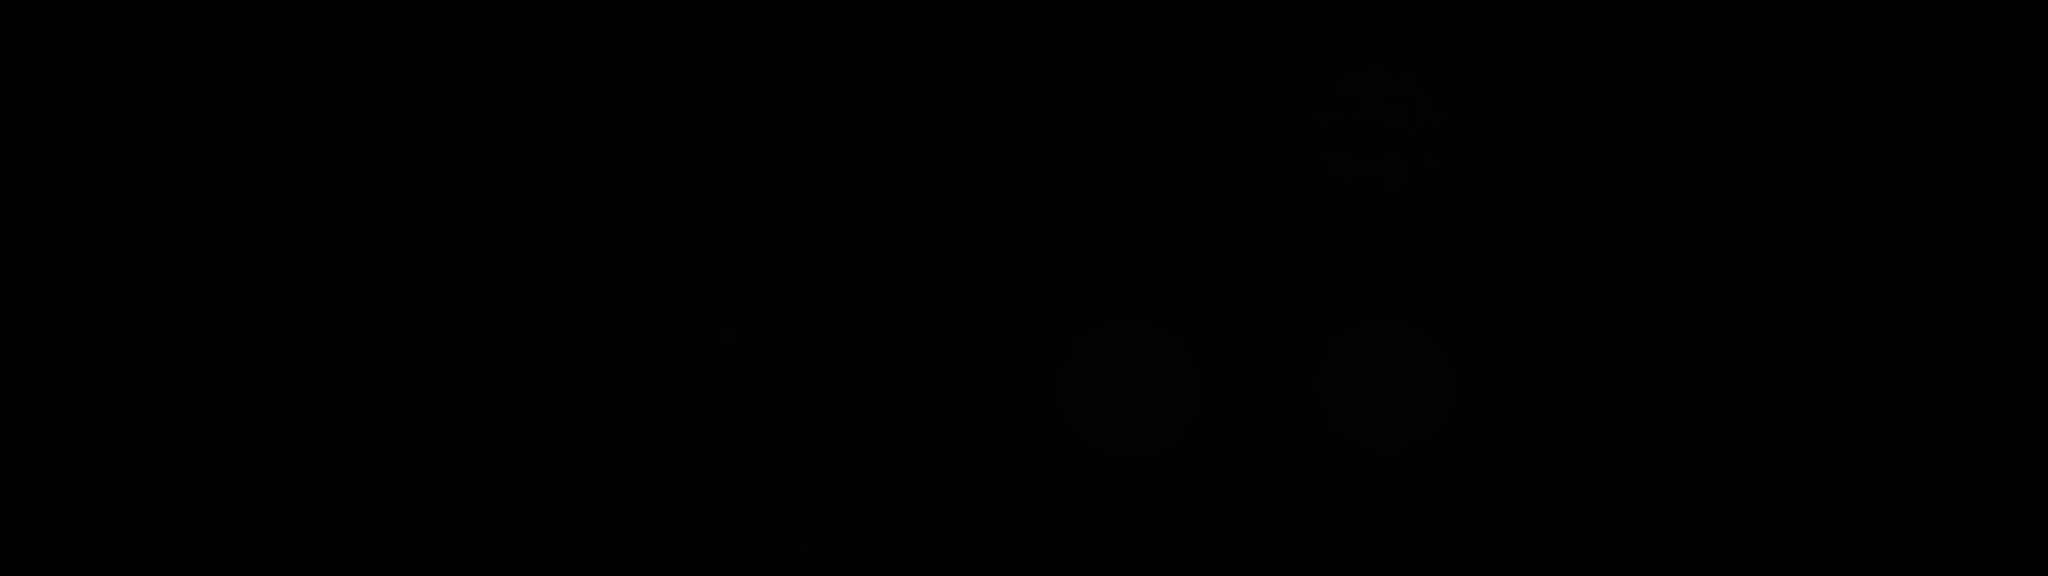
\includegraphics[height=0.023\textheight]{spatial-denoised/wavelet_den_30.png}\\
        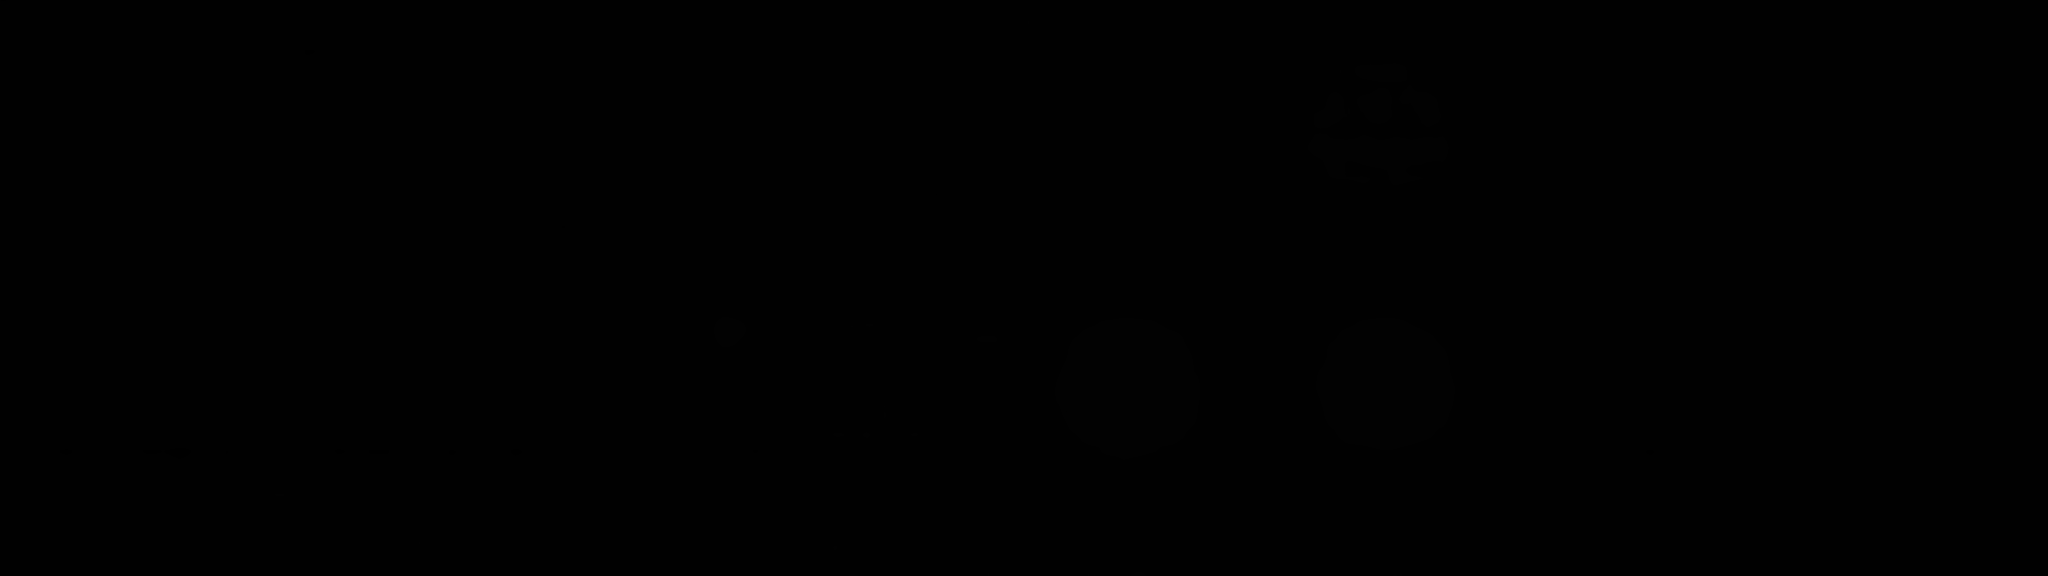
\includegraphics[height=0.023\textheight]{spatial-denoised/wavelet_den_31.png}
        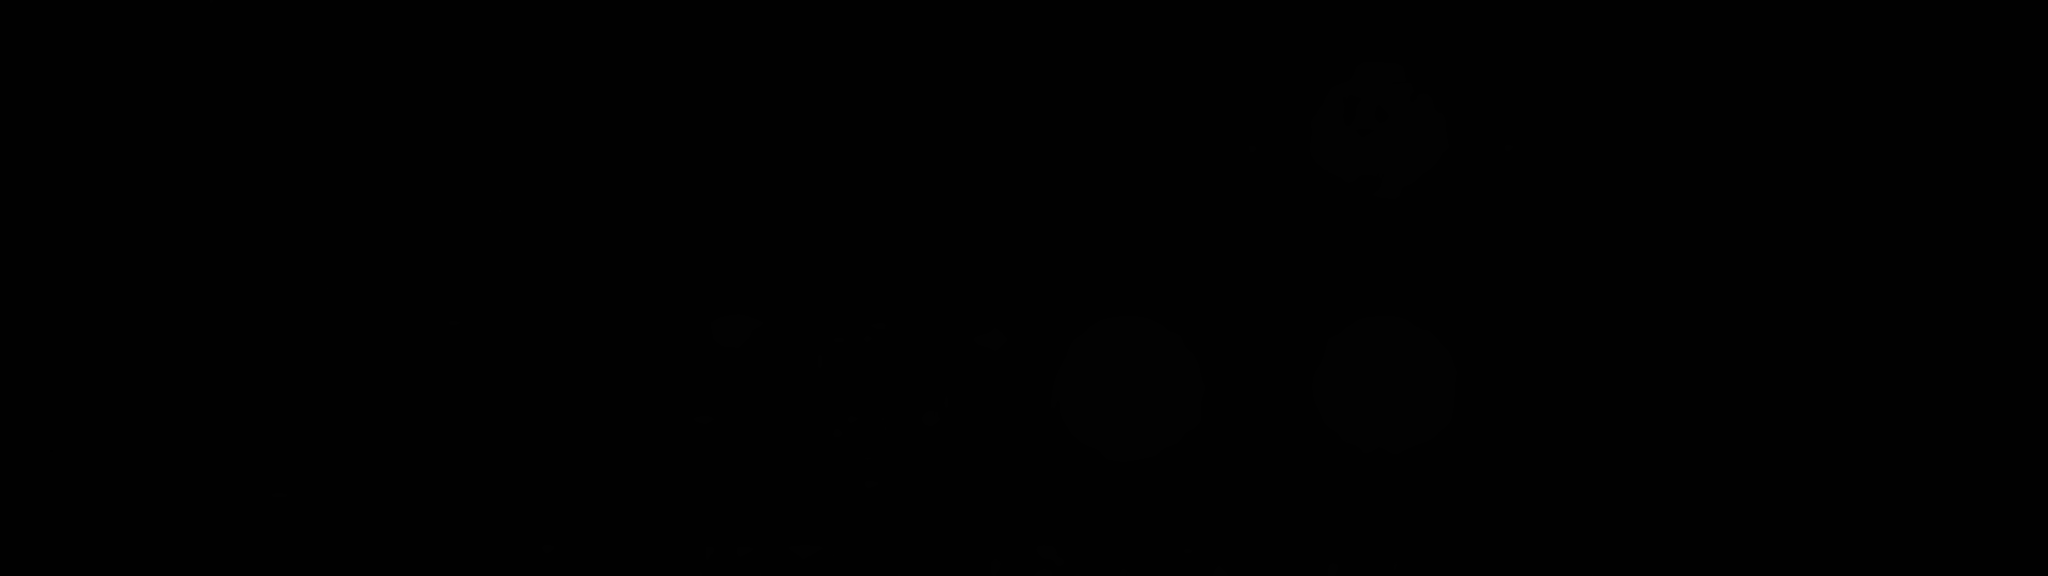
\includegraphics[height=0.023\textheight]{spatial-denoised/wavelet_den_32.png}
        
\includegraphics[height=0.023\textheight]{spatial-denoised/wavelet_den_33.png}
        
\includegraphics[height=0.023\textheight]{spatial-denoised/wavelet_den_34.png}
        
\includegraphics[height=0.023\textheight]{spatial-denoised/wavelet_den_35.png}
        
\includegraphics[height=0.023\textheight]{spatial-denoised/wavelet_den_36.png}
        
\includegraphics[height=0.023\textheight]{spatial-denoised/wavelet_den_37.png}
        
\includegraphics[height=0.023\textheight]{spatial-denoised/wavelet_den_38.png}
        \includegraphics[height=0.023\textheight]{spatial-denoised/wavelet_den_39.png}
        \includegraphics[height=0.023\textheight]{spatial-denoised/wavelet_den_40.png}
        \includegraphics[height=0.023\textheight]{spatial-denoised/wavelet_den_41.png}
        \includegraphics[height=0.023\textheight]{spatial-denoised/wavelet_den_42.png}
        \includegraphics[height=0.023\textheight]{spatial-denoised/wavelet_den_43.png}
        \includegraphics[height=0.023\textheight]{spatial-denoised/wavelet_den_44.png}
        \includegraphics[height=0.023\textheight]{spatial-denoised/wavelet_den_45.png}\\
        \includegraphics[height=0.023\textheight]{spatial-denoised/wavelet_den_46.png}
        \includegraphics[height=0.023\textheight]{spatial-denoised/wavelet_den_47.png}
        \includegraphics[height=0.023\textheight]{spatial-denoised/wavelet_den_48.png}
        \includegraphics[height=0.023\textheight]{spatial-denoised/wavelet_den_49.png}
        \includegraphics[height=0.023\textheight]{spatial-denoised/wavelet_den_50.png}
        \includegraphics[height=0.023\textheight]{spatial-denoised/wavelet_den_51.png}
        \includegraphics[height=0.023\textheight]{spatial-denoised/wavelet_den_52.png}
        \includegraphics[height=0.023\textheight]{spatial-denoised/wavelet_den_53.png}
        \includegraphics[height=0.023\textheight]{spatial-denoised/wavelet_den_54.png}
        \includegraphics[height=0.023\textheight]{spatial-denoised/wavelet_den_55.png}
        \includegraphics[height=0.023\textheight]{spatial-denoised/wavelet_den_56.png}
        \includegraphics[height=0.023\textheight]{spatial-denoised/wavelet_den_57.png}
        \includegraphics[height=0.023\textheight]{spatial-denoised/wavelet_den_58.png}
        \includegraphics[height=0.023\textheight]{spatial-denoised/wavelet_den_59.png}
        \includegraphics[height=0.023\textheight]{spatial-denoised/wavelet_den_60.png}\\
        \includegraphics[height=0.023\textheight]{spatial-denoised/wavelet_den_61.png}
        \includegraphics[height=0.023\textheight]{spatial-denoised/wavelet_den_62.png}
        \includegraphics[height=0.023\textheight]{spatial-denoised/wavelet_den_62.png}
        \includegraphics[height=0.023\textheight]{spatial-denoised/wavelet_den_63.png}
        \includegraphics[height=0.023\textheight]{spatial-denoised/wavelet_den_64.png}
        \includegraphics[height=0.023\textheight]{spatial-denoised/wavelet_den_64.png}
        \includegraphics[height=0.023\textheight]{spatial-denoised/wavelet_den_65.png}
        \includegraphics[height=0.023\textheight]{spatial-denoised/wavelet_den_66.png}
        \includegraphics[height=0.023\textheight]{spatial-denoised/wavelet_den_67.png}
        \includegraphics[height=0.023\textheight]{spatial-denoised/wavelet_den_68.png}
        \includegraphics[height=0.023\textheight]{spatial-denoised/wavelet_den_69.png}
        \includegraphics[height=0.023\textheight]{spatial-denoised/wavelet_den_70.png}
        \includegraphics[height=0.023\textheight]{spatial-denoised/wavelet_den_71.png}
        \includegraphics[height=0.023\textheight]{spatial-denoised/wavelet_den_72.png}

        \vspace{1mm}
        \includegraphics[scale=0.1]{spatial-denoised/wavelet_den_45.png}

        \vspace{1mm}
        \includegraphics[scale=0.25]{contrastAgentResponses1.png} 

\end{frame}


\begin{frame}
    \frametitle{References}
\end{frame}


\end{document} 